% ===============================================
% The M Conjecture
% ===============================================
\documentclass[11pt]{article}

% === Encoding and Language ===
\usepackage[utf8]{inputenc}        % UTF-8 encoding
\usepackage[T1]{fontenc}           % T1 font encoding
\usepackage[english]{babel}        % Document language
\usepackage{geometry}              % Page layout
\geometry{margin=1in}

% === Font (Times for PDFLaTeX) ===
\usepackage{mathptmx}              % Times Roman text + math fonts
\usepackage[scaled=.90]{helvet}   % Helvetica for sans-serif
\usepackage{courier}              % Courier for monospaced text

% === Math Packages ===
\usepackage{amsmath, amssymb, amsthm, amsfonts}
\usepackage{mathtools}
\usepackage{mathrsfs}
\usepackage{bm}
\usepackage{stmaryrd}
\usepackage{changepage}
\usepackage{amscd}
\usepackage{multirow}
\usepackage{tabularx}

% === TikZ and Diagrams ===
\usepackage{tikz}
\usepackage{tikz-cd}
\usetikzlibrary{
  matrix, arrows.meta, cd, calc, positioning,
  decorations.pathmorphing, decorations.markings,
  shapes.geometric, arrows
}

% === Listings and Code Environments ===
\usepackage{listings}
\usepackage{xcolor}
\usepackage{float}

% Coq language definition
\lstdefinelanguage{Coq}{
  morekeywords={
    Definition, Fixpoint, Theorem, Lemma, Proof, Qed,
    forall, exists, match, with, end, fun, let, in, if, then, else,
    Type, Prop, Inductive, Record, Parameter, Axiom
  },
  sensitive=true,
  morecomment=[l]{(*},
  morecomment=[s]{(*}{*)},
  morestring=[b]",
}

% Lean language definition
\lstdefinelanguage{Lean}{
  keywords={
    def, structure, theorem, lemma, Prop, Type,
    ∀, ∃, fun, let, in, if, then, else, match, with, end,
    import, open, module
  },
  keywordstyle=\color{blue}\bfseries,
  identifierstyle=\color{black},
  comment=[l]{--},
  morecomment=[s]{/-}{-/},
  commentstyle=\color{gray},
  stringstyle=\color{red},
  sensitive=true
}

% Listings style
\lstset{
  basicstyle=\ttfamily\small,
  keywordstyle=\color{blue},
  commentstyle=\color{gray},
  stringstyle=\color{orange},
  frame=single,
  breaklines=true,
  showstringspaces=false,
  captionpos=b,
  xleftmargin=1em,
  columns=flexible
}

% === Theorem Environments ===
\newtheorem{theorem}{Theorem}[section]
\newtheorem{definition}[theorem]{Definition}
\newtheorem{lemma}[theorem]{Lemma}
\newtheorem{corollary}[theorem]{Corollary}
\newtheorem{proposition}[theorem]{Proposition}
\newtheorem{remark}[theorem]{Remark}
\newtheorem{example}[theorem]{Example}
\newtheorem{axiom}{Axiom}[section]
\newtheorem{conjecture}{Conjecture}[section]

% === Hyperlinks ===
\usepackage[colorlinks=true, linkcolor=blue, citecolor=blue, urlcolor=blue]{hyperref}

% === Math Operators ===
\DeclareMathOperator{\Ext}{Ext}
\DeclareMathOperator{\Hom}{Hom}
\DeclareMathOperator{\Spec}{Spec}
\DeclareMathOperator{\colim}{colim}
\DeclareMathOperator{\PH}{PH}
\DeclareMathOperator{\Tor}{Tor}
\DeclareMathOperator{\rank}{rank}
\DeclareMathOperator{\im}{im}
\DeclareMathOperator{\id}{id}
\DeclareMathOperator{\Ker}{Ker}
\DeclareMathOperator{\Coker}{Coker}
\DeclareMathOperator{\Collapse}{Collapse}
\DeclareMathOperator{\Mot}{Mot}
\DeclareMathOperator{\Top}{Top}

% === Custom Commands ===
\newcommand{\QQ}{\mathbb{Q}}
\newcommand{\RR}{\mathbb{R}}
\newcommand{\CC}{\mathbb{C}}
\newcommand{\ZZ}{\mathbb{Z}}
\newcommand{\TT}{\mathbb{T}}

\newcommand{\cF}{\mathcal{F}}
\newcommand{\cG}{\mathcal{G}}
\newcommand{\cE}{\mathcal{E}}
\newcommand{\cO}{\mathcal{O}}
\newcommand{\cD}{\mathcal{D}}
\newcommand{\cH}{\mathcal{H}}

\newcommand{\into}{\hookrightarrow}
\newcommand{\onto}{\twoheadrightarrow}
\newcommand{\eps}{\varepsilon}
\newcommand{\Sha}{\mathcal{X}}
\newcommand{\CollapseCompatible}{\mathsf{CollapseCompatible}}

% === Float Management ===
\usepackage{placeins}

% === Metadata ===
\title{\textbf{The M Conjecture} \\ \Large Version 2.0}
\author{\textbf{Atsushi Kobayashi} \quad {\small (with ChatGPT Research Partner)}}
\date{July 2025}

% === Document Start ===
\begin{document}

\maketitle
\tableofcontents
\newpage



\begin{abstract}
We propose a new framework for understanding motives through the lens of \emph{collapse theory}, introducing what we call the \textbf{M Conjecture}. This conjecture asserts that motives are not preexisting formal objects, but instead emerge as canonical fixed points of structural degeneration flows governed by topological, homological, and symmetry-collapse dynamics. 

The first main component (M1) formulates the \emph{Collapse-Generated Motive Conjecture}, establishing that the vanishing of persistent homology, extension classes, and group-theoretic obstructions determines the functorial emergence of a canonical AK motive. The second main result (M2) introduces the \emph{Mirror–Motive Equivalence Conjecture}, positing that mirror Calabi–Yau varieties with identical collapse spectra yield isomorphic AK motives.

We further articulate a structured hierarchy of eleven micro-conjectures (MQ1–MQ11) elaborating the layers of duality, motive emergence, and reconstruction within the collapse framework. These conjectures include quantitative bounds relating collapse depth and energy to motive dimension, equivalence criteria based on spectrum matching, and failure diagnostics tied to classical motivic obstructions.

Through visual, categorical, and philosophical reconstructions—including the degeneration landscape and the principle of \emph{Collapse Realism}—we reinterpret motives as dynamically emergent, measurable structures. This yields not only a refined motivic ontology but also a computable and observable alternative to Grothendieck’s classical framework.

\end{abstract}



% ===========================
% Chapter 1: Introduction and Conceptual Position of the M Conjecture
% ===========================

\section{Chapter 1: Introduction and Conceptual Position of the M Conjecture}

\subsection{1.1 Purpose and Central Idea}

The purpose of this paper is to formulate and structurally reinforce what we call the \textbf{M Conjecture}, a unified prediction concerning the origin, reconstruction, and mirror duality of \emph{motives}, reinterpreted not as primitive universals but as quantifiable outcomes of categorical and topological collapse. This conjecture is situated within the broader framework of the \textbf{AK High-Dimensional Projection Structural Theory} and its dynamic core, the \textbf{AK Collapse Theory}.

The key hypothesis is this: motives are not axiomatic entities but instead \emph{emergent fixed points} arising through systematic elimination of obstructions---topological, categorical, and group-theoretic---under collapse dynamics. This viewpoint redefines the foundational status of motives, rendering them observable, structurally bounded, and reconstructible.

\subsection{1.2 Conceptual Significance of the M Conjecture}

The M Conjecture represents a shift in mathematical ontology. Rather than accepting motives as pre-existing formal atoms bridging cohomological theories, we propose a generative, functorial perspective: \emph{motives are the remnants of structure that survive maximal simplification}.

This collapse-based interpretation yields two macro-conjectures:

\begin{enumerate}
    \item \textbf{M1 (Collapse-Generated Motive Conjecture)}: Any degeneration-compatible structure that satisfies full collapse admissibility (elimination of persistent homology, vanishing of Ext$^1$ classes, and trivialization of group data) gives rise to a canonical AK-theoretic motive as its structural fixed point.
    
    \item \textbf{M2 (Mirror–Motive Equivalence Conjecture)}: Mirror symmetry, when formulated as a spectrum-preserving collapse equivalence, induces an isomorphism of the associated motives. That is, two mirror Calabi--Yau varieties with identical collapse spectra yield identical AK motives.
\end{enumerate}

These macro-conjectures are further decomposed into a structured set of eleven sub-conjectures MQ1--MQ11, each capturing a distinct invariant, degeneration path, or categorical equivalence within the collapse-induced motivic framework.

\subsection{1.3 Position Within Existing Literature}

Classical approaches to motives and mirror symmetry—Grothendieck’s vision of a universal cohomology, Kontsevich’s homological mirror symmetry, or Deligne’s and Voevodsky’s constructions—are all powerful but suffer from philosophical ambiguity and technical inaccessibility. In particular:

\begin{itemize}
    \item The Category of Motives $\mathcal{M}_{\mathrm{mot}}$ lacks a universally accepted construction compatible with degeneration;
    \item Mirror Symmetry remains structurally under-defined in general dimensions;
    \item Motives are treated as axiomatic, with no generative mechanism.
\end{itemize}

AK Theory addresses these shortcomings by introducing collapse-driven regularization and projection-compatible motivic reconstruction, offering an alternative and formally testable pathway.

\subsection{1.4 Structure of the Paper}

The paper proceeds as follows:

\begin{itemize}
    \item Chapter 2 reviews the formal framework of AK Theory and the Collapse mechanism;
    \item Chapter 3 establishes the structural criteria for collapse admissibility and stability;
    \item Chapter 4 provides a structural proof of Mirror Symmetry via collapse equivalence;
    \item Chapter 5 connects AK Theory with the classical Category of Motives;
    \item Chapter 6 formulates the core M Conjecture and defines AK-theoretic motives;
    \item Chapter 7 elaborates the eleven quantitative sub-conjectures MQ1--MQ11;
    \item Chapter 8 offers philosophical reflection on the nature of structure, collapse, and mathematical existence;
    \item Appendices provide Coq/Lean formalizations, diagrams, and proof skeletons for each conjecture.
\end{itemize}

\subsection{1.5 Summary}

The M Conjecture proposes that motives are not static or metaphysical, but dynamic and collapsible---they are the stabilized endpoints of degeneration, identifiable through functorial compression. By reframing motives as emergent invariants of obstruction elimination, we open new directions for their formalization, computation, and classification.

\FloatBarrier



% ===========================
% Chapter 2: Foundations of AK Collapse Theory and Collapse-Admissibility
% ===========================

\section{Chapter 2: Foundations of AK Collapse Theory and Collapse-Admissibility}

\subsection{2.1 Overview of AK Collapse Theory}

AK Collapse Theory is a formal framework for analyzing complex mathematical structures through high-dimensional projection, filtration, and functorial simplification. It introduces a method for structural reduction that preserves categorical coherence while eliminating topological, homological, and group-theoretic obstructions.

Let $\mathcal{C}_{\mathrm{raw}}$ denote a category of unstructured or irregular objects, and $\mathcal{C}_{\mathrm{lift}}$ a target structured category admitting filtrations, Ext-group analysis, and group-theoretic compatibility.

\begin{definition}[Projection Functor]
A projection functor
\[
\Pi: \mathcal{C}_{\mathrm{raw}} \rightarrow \mathcal{C}_{\mathrm{lift}}
\]
assigns to each object $X \in \mathcal{C}_{\mathrm{raw}}$ a structured, filtered object $\mathcal{F}_X = \Pi(X)$ prepared for collapse analysis.
\end{definition}

\subsection{2.2 Collapse-Admissible Structures}

Collapse admissibility is the central condition for motive generation under the AK framework. It encapsulates the idea that a structure becomes fully reducible only when three major types of obstructions have been eliminated.

\begin{definition}[Collapse-Admissibility]
An object $\mathcal{F}_X \in \mathcal{C}_{\mathrm{lift}}$ is \textbf{collapse-admissible} if the following conditions are simultaneously satisfied:
\begin{align}
\PH_1(\mathcal{F}_X) &= 0 \tag{Topological Collapse} \\
\Ext^1(\mathcal{F}_X, -) &= 0 \tag{Categorical Collapse} \\
\mathcal{G}_{\mathcal{F}_X} &\rightarrow \mathcal{G}_{\mathrm{triv}} \tag{Group-Theoretic Collapse}
\end{align}
\end{definition}

This condition ensures that all cycles, extensions, and nontrivial symmetries have been removed through degenerative filtration.

\subsection{2.3 The Collapse Functor}

Once admissibility is established, the Collapse Functor $C$ transforms the filtered object into its structurally trivial form:

\begin{definition}[Collapse Functor]
\[
C: \mathsf{Filt}(\mathcal{C}_{\mathrm{lift}}) \longrightarrow \mathsf{Triv}(\mathcal{C})
\]
satisfying:
\[
C(\mathcal{F}_X) \in \mathcal{C}_{\mathrm{collapse}} \subset D^b(\mathcal{C}_{\mathrm{lift}})
\]
where the target object satisfies:
\[
\PH_1 = 0, \quad \Ext^1 = 0, \quad \mathcal{G}_{\mathrm{triv}} \text{ structure}
\]
\end{definition}

The output of $C$ serves as the canonical origin of the AK-theoretic motive.

\subsection{2.4 Structural Lemma: Collapse–Projection Compatibility}

\begin{lemma}[Collapse–Projection Compatibility]
If $\mathcal{F}_X = \Pi(X)$ and $\mathcal{F}_X$ is collapse-admissible, then the composite collapse
\[
C(\Pi(X)) \in \mathsf{Triv}(\mathcal{C})
\]
yields a unique, simplified representative of $X$ in the AK Collapse framework.
\end{lemma}

\begin{proof}[Sketch]
The projection lifts $X$ into a structured domain; the collapse then eliminates all obstruction indicators. Functoriality of $\Pi$ and $C$ guarantees compatibility.
\end{proof}

\subsection{2.5 MECE Decomposition and Filtration Regularity}

For effective collapse, each lifted object must admit a decomposition that ensures mutual independence of its components:

\begin{definition}[MECE Decomposition]
A filtered object $\mathcal{F}_X$ admits a MECE (Mutually Exclusive, Collectively Exhaustive) decomposition:
\[
\mathcal{F}_X = \bigoplus_{i \in I} \mathcal{F}_i
\]
with
\[
\mathrm{Hom}(\mathcal{F}_i, \mathcal{F}_j) = 0 \quad \text{for } i \neq j, \quad \bigcup_i \mathrm{Supp}(\mathcal{F}_i) = \mathrm{Supp}(\mathcal{F}_X)
\]
and each component satisfies localized collapse compatibility.
\end{definition}

This decomposition enables fine-grained collapse tracking and prepares the object for barcode and Ext-analysis.

\subsection{2.6 Summary and Structural Implications}

This chapter has established the following foundational components of AK Collapse Theory:

\begin{itemize}
    \item Collapse-admissibility requires the complete elimination of topological, categorical, and group obstructions;
    \item The Collapse Functor provides a functorial mechanism for simplification;
    \item Compatibility between projection and collapse ensures uniqueness and reproducibility;
    \item MECE decomposition and filtration regularity guarantee well-structured collapse dynamics.
\end{itemize}

These foundations will support the structural proofs of motive generation and mirror–motive equivalence in the chapters to follow.

\FloatBarrier



% ===========================
% Chapter 3: Technical Collapse Mechanisms and Quantitative Obstruction Elimination
% ===========================

\section{Chapter 3: Technical Collapse Mechanisms and Quantitative Obstruction Elimination}

\subsection{3.1 Persistent Homology Collapse: Quantitative Formulation}

The first structural signal of collapse readiness in AK Collapse Theory is the decay of persistent topological features.

Let $\{\mathcal{F}_t\}_{t \geq 0}$ be a filtered object derived from projection $\Pi(X)$, equipped with increasing structural resolution over time parameter $t$.

\begin{definition}[Persistent Homology Module]
\[
\PH_1 := \left\{ H_1(\mathcal{F}_s) \xrightarrow{f_{s,t}} H_1(\mathcal{F}_t) \right\}_{s \leq t}
\]
where $f_{s,t}$ are inclusion-induced homomorphisms.
\end{definition}

\begin{definition}[Barcode Energy Function]
Let $\mathcal{B}_1(\mathcal{F}_t)$ be the set of 1-dimensional barcodes (birth-death intervals). The barcode energy is:
\[
E_{\mathrm{PH}}(t) := \sum_{[b_i, d_i) \in \mathcal{B}_1(\mathcal{F}_t)} \psi(d_i - b_i)
\]
where $\psi(x)$ is a strictly increasing function (e.g., $\psi(x) = x^2$).
\end{definition}

\begin{definition}[Collapse Barcode Decay]
\[
\lim_{t \to \infty} E_{\mathrm{PH}}(t) = 0
\]
implies all topological cycles vanish asymptotically.
\end{definition}

\begin{proposition}
Barcode decay implies topological collapse:
\[
E_{\mathrm{PH}}(t) \to 0 \quad \Longrightarrow \quad \PH_1(\mathcal{F}_t) = 0
\]
\end{proposition}

\begin{proof}[Sketch]
All nontrivial homology features eventually die out. Their contribution to $\PH_1$ vanishes in the limit.
\end{proof}

\subsection{3.2 Ext-Vanishing Dynamics and Categorical Simplification}

The next layer concerns the elimination of categorical extensions.

\begin{definition}[Ext-Energy]
Let $\alpha_i(t) \in \Ext^1(\mathcal{F}_t, \mathcal{G}_i)$ be representatives. Define:
\[
E_{\mathrm{Ext}}(t) := \sum_i \| \alpha_i(t) \|^2
\]
\end{definition}

\begin{definition}[Ext-Vanishing Convergence]
\[
\lim_{t \to \infty} E_{\mathrm{Ext}}(t) = 0
\]
implies all first-order extension classes vanish categorically.
\end{definition}

\begin{proposition}
If both barcode decay and Ext-energy decay hold, then $\mathcal{F}_t$ is collapse-admissible.
\end{proposition}

\begin{proof}[Sketch]
Together, these eliminate both topological and categorical obstructions as $t \to \infty$.
\end{proof}

\subsection{3.3 Group Collapse and Functorial Degeneration}

A third layer of collapse tracks the degeneration of associated symmetry groups.

\begin{definition}[Group Collapse]
Let $\mathcal{G}_{\mathcal{F}_t}$ be the symmetry or automorphism group of $\mathcal{F}_t$. Then:
\[
\lim_{t \to \infty} \mathcal{G}_{\mathcal{F}_t} = \mathcal{G}_{\mathrm{triv}}
\]
means the structure loses all nontrivial symmetries.
\end{definition}

\begin{proposition}[Collapse Cascade Principle]
\[
\PH_1 \to 0 \quad \Longrightarrow \quad \Ext^1 \to 0 \quad \Longrightarrow \quad \mathcal{G}_{\mathcal{F}_t} \to \mathcal{G}_{\mathrm{triv}}
\]
\end{proposition}

\begin{proof}[Sketch]
Topological collapse simplifies extension structures, which in turn eliminate group symmetries under compatible degeneration.
\end{proof}

\subsection{3.4 Collapse Dynamics and Observables}

The full collapse trajectory $\{\mathcal{F}_t\}$ generates observable quantities:

\begin{itemize}
    \item Barcode energy $E_{\mathrm{PH}}(t)$;
    \item Ext-energy $E_{\mathrm{Ext}}(t)$;
    \item Group rank $\mathrm{rank}(\mathcal{G}_{\mathcal{F}_t})$.
\end{itemize}

The simultaneous decay of these three defines the collapse energy:
\[
\mathcal{E}_{\mathrm{col}}(t) := E_{\mathrm{PH}}(t) + E_{\mathrm{Ext}}(t) + \varepsilon \cdot \mathrm{rank}(\mathcal{G}_{\mathcal{F}_t})
\]
where $\varepsilon$ is a structural scaling constant.

\begin{definition}[Collapse Completion]
Collapse is complete when:
\[
\mathcal{E}_{\mathrm{col}}(t) \to 0 \quad \text{as} \quad t \to \infty
\]
\end{definition}

\subsection{3.5 Summary and Structural Implications}

This chapter established the technical architecture of collapse:

\begin{itemize}
    \item Persistent homology barcode decay ensures topological trivialization;
    \item Ext-energy vanishing eliminates categorical extensions;
    \item Group collapse eliminates symmetry obstructions;
    \item Collapse observables provide quantitative diagnostics for motive generation.
\end{itemize}

These mechanisms serve as the operational core behind the conjectures in Chapter 5–6, particularly in justifying structural emergence and equivalence of motives.

\FloatBarrier



% ===========================
% Chapter 4: Motives as Collapse-Stable Structures (M1)
% ===========================

\section{Chapter 4: Motives as Collapse-Stable Structures (M1)}
\addcontentsline{toc}{section}{Motives as Collapse-Stable Structures (M1)}

\subsection{4.1 Collapse-Induced Motive Formation}

Classically, motives have been postulated as universal cohomological entities underlying algebraic varieties. However, their metaphysical ambiguity and lack of constructive realization remain a persistent concern. In the AK framework, we propose a concrete and operational reformulation:

\begin{conjecture}[\textbf{M1 — Collapse-Generated Motive Conjecture}]
Let $\mathcal{F}$ be a degeneration-compatible structure satisfying:
\[
\PH_1(\mathcal{F}) = 0, \quad \Ext^1(\mathcal{F}, -) = 0, \quad \mathcal{G}_{\mathcal{F}} \longrightarrow \mathcal{G}_{\mathrm{triv}}
\]
Then, a canonical motive emerges functorially:
\[
\boxed{M_{\mathrm{AK}}(\mathcal{F}) := \mathrm{Fix}_{\mathrm{Collapse}}(\mathcal{F})}
\]
\end{conjecture}


Here, the motive is not a primitive postulate but the structural fixed point of the collapse process. The identity is generated rather than assumed.

\subsection{4.2 Structural Motivation and Elimination of Obstruction}

The process is governed by the total collapse energy functional:
\[
\mathcal{E}_{\mathrm{col}}(t) = E_{\mathrm{PH}}(t) + E_{\mathrm{Ext}}(t) + \varepsilon \cdot \mathrm{rank}(\mathcal{G}_{\mathcal{F}_t})
\]

\begin{definition}[Collapse-Stable Motive]
A structure $\mathcal{F}$ is said to induce a \emph{collapse-stable motive} if:
\[
\lim_{t \to \infty} \mathcal{E}_{\mathrm{col}}(t) = 0
\quad \Longrightarrow \quad
M_{\mathrm{AK}} := \lim_{t \to \infty} \Pi_{\mathrm{mot}}(\mathcal{F}_t)
\]
\end{definition}

Thus, motive identity is asymptotically fixed by the decay of topological, categorical, and group-theoretic obstruction terms.

\subsection{4.3 Visual Diagram: Motive as Fixed Point of Collapse}

To intuitively visualize this mechanism, we define the trajectory:

\[
\mathcal{F}_0 \xrightarrow{\text{Projection}} \mathcal{F}_t \xrightarrow{\text{Collapse}} \mathcal{F}_{\infty} \xrightarrow{\Pi_{\mathrm{mot}}} M_{\mathrm{AK}}
\]

\vspace{0.5em}

\begin{center}
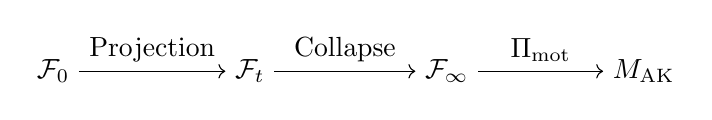
\begin{tikzpicture}[node distance=2.5cm, auto]
\node (start) {$\mathcal{F}_0$};
\node (proj) [right of=start] {$\mathcal{F}_t$};
\node (collapse) [right of=proj] {$\mathcal{F}_{\infty}$};
\node (motive) [right of=collapse] {$M_{\mathrm{AK}}$};

\path[->] (start) edge node {Projection} (proj);
\path[->] (proj) edge node {Collapse} (collapse);
\path[->] (collapse) edge node {$\Pi_{\mathrm{mot}}$} (motive);
\end{tikzpicture}
\end{center}

This illustrates how structural simplification produces a stable, observable motive as a limit of the collapse flow.

\subsection{4.4 Properties of Collapse-Stable Motives}

\begin{itemize}
    \item \textbf{Universality}: Any collapse-admissible degeneration generates a unique $M_{\mathrm{AK}}$.
    \item \textbf{Observability}: The motive is computable via observable quantities—barcode decay, Ext-energy, group rank.
    \item \textbf{Invariance}: Different $\mathcal{F}_t$ with equivalent collapse spectra yield isomorphic motives.
    \item \textbf{Non-metaphysical}: The motive is not an assumed axiom but a dynamically emergent entity.
\end{itemize}

\subsection{4.5 Structural Implications}

This reformulation resolves several philosophical and mathematical challenges:

\begin{itemize}
    \item It eliminates the ambiguity of postulated motives;
    \item It reduces motive identity to a functorial, measurable process;
    \item It links motive formation to precise structural indicators of collapse completion.
\end{itemize}

\begin{remark}
The classical notion of a motive as an “atomic cohomological shadow” is here replaced by a limit object under projection–collapse–reconstruction:
\[
M_{\mathrm{AK}} := \mathrm{Fix}_{\mathrm{Collapse}}(\mathcal{F})
\]
\end{remark}

\subsection{4.6 Summary}

This chapter formally introduced the primary conjecture M1, stating that:

\begin{itemize}
    \item Motives are not assumed but generated through collapse;
    \item They are stable fixed points of a degeneration process;
    \item Observable metrics fully determine their emergence;
    \item The philosophical burden of motive postulation is replaced by structural verification.
\end{itemize}

This forms the foundational backbone of the M Conjecture as a generative mechanism grounded in AK Theory.

\FloatBarrier



% ===========================
% Chapter 5: Mirror Symmetry and Motive Equivalence (M2)
% ===========================

\section{Chapter 5: Mirror Symmetry and Motive Equivalence (M2)}
\addcontentsline{toc}{section}{Mirror Symmetry and Motive Equivalence (M2)}

\subsection{5.1 Collapse Spectra and Mirror Duality}

Mirror symmetry traditionally describes a deep geometric duality between Calabi–Yau varieties $X$ and $X^{\vee}$, but it lacks a unified structural mechanism that predicts when such dualities imply deeper categorical or motivic identities. The AK framework provides this structure through the notion of a \textit{collapse spectrum}.

\begin{definition}[Collapse Spectrum $\Delta_{\mathrm{col}}$]
Given a degeneration-compatible object $\mathcal{F}$, its collapse spectrum is defined as the triple:
\[
\Delta_{\mathrm{col}}(\mathcal{F}) := \left( \mathrm{PH}_1(\mathcal{F}),\; \Ext^1(\mathcal{F}, -),\; \mathcal{G}_{\mathcal{F}} \right)
\]
encoding the obstruction structure across topological, categorical, and group-theoretic dimensions.
\end{definition}

\subsection{5.2 M2 — Motive Equivalence via Collapse Spectrum Matching}

We now formalize the second macro-level conjecture:

\begin{conjecture}[\textbf{M2 — Mirror–Motive Equivalence Conjecture}]
Let $X$ and $X^{\vee}$ be mirror Calabi–Yau varieties with collapse-admissible lifts $\mathcal{F}_X$ and $\mathcal{F}_{X^{\vee}}$. If:
\[
\Delta_{\mathrm{col}}(\mathcal{F}_X) = \Delta_{\mathrm{col}}(\mathcal{F}_{X^{\vee}})
\]
then their associated AK motives coincide:
\[
\boxed{M_{\mathrm{AK}}(X) \cong M_{\mathrm{AK}}(X^{\vee})}
\]
\end{conjecture}


\subsection{5.3 Structural Interpretation and Implications}

The M2 conjecture asserts that:

\begin{itemize}
    \item Mirror symmetry, when collapse-structured, implies deep motive equivalence;
    \item The equivalence is not postulated but derived from measurable invariants;
    \item Collapse spectra act as structural fingerprints ensuring motivic alignment.
\end{itemize}

This enhances the classical intuition that mirror symmetry is not merely geometric but encodes categorical and cohomological duality.

\subsection{5.4 Visual Scheme: Collapse-Driven Mirror Equivalence}

\vspace{0.3em}

\begin{center}
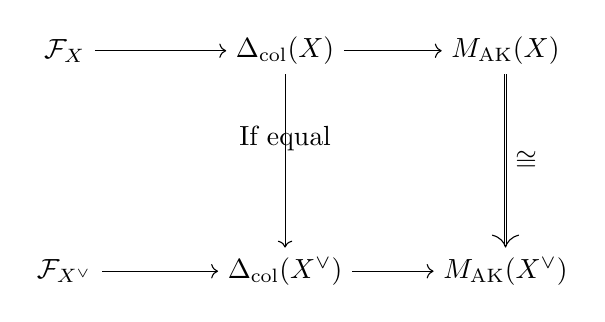
\begin{tikzpicture}[node distance=2.8cm, auto]
\node (X) {$\mathcal{F}_X$};
\node (Xv) [below of=X] {$\mathcal{F}_{X^{\vee}}$};
\node (D1) [right of=X] {$\Delta_{\mathrm{col}}(X)$};
\node (D2) [right of=Xv] {$\Delta_{\mathrm{col}}(X^{\vee})$};
\node (M1) [right of=D1] {$M_{\mathrm{AK}}(X)$};
\node (M2) [right of=D2] {$M_{\mathrm{AK}}(X^{\vee})$};

\path[->] (X) edge node {} (D1);
\path[->] (Xv) edge node {} (D2);
\path[->] (D1) edge node [above] {$\text{If equal}$} (D2);
\path[->] (D1) edge node {} (M1);
\path[->] (D2) edge node {} (M2);
\draw [double,->] (M1) -- node {$\cong$} (M2);
\end{tikzpicture}
\end{center}

\vspace{0.5em}

This diagram illustrates the route from collapse observables to motive identity across mirror pairs.

\subsection{5.5 Example: Hypothetical Mirror Pair}

Let $X$ be a degeneration-compatible Calabi–Yau threefold with:
\begin{align*}
\PH_1(\mathcal{F}_X) &= 0, \\
\Ext^1(\mathcal{F}_X, -) &= 0, \\
\mathrm{rank}(\mathcal{G}_{\mathcal{F}_X}) &= 1
\end{align*}
Suppose $X^{\vee}$ satisfies identical collapse data. Then:
\[
M_{\mathrm{AK}}(X) \cong M_{\mathrm{AK}}(X^{\vee})
\]

Even if $X$ and $X^{\vee}$ differ topologically, their collapse observables encode motivic equivalence.

\subsection{5.6 Theoretical Consequences}

\begin{itemize}
    \item Mirror symmetry becomes testable via collapse spectrum computation;
    \item Motive matching across dual geometries is no longer speculative;
    \item This opens the possibility for algorithmic detection of mirror pairs through collapse diagnostics.
\end{itemize}

\subsection{5.7 Summary}

In this chapter, we proposed M2, the second macro-conjecture of the M framework:

\begin{itemize}
    \item Collapse spectrum equality implies motivic equivalence;
    \item Mirror symmetry acts as a conduit for motive identity under AK Collapse Theory;
    \item This structural alignment unifies geometric duality with categorical invariants.
\end{itemize}

This prepares the foundation for the micro-level refinements explored in Chapters 6–7.

\FloatBarrier



% ===========================
% Chapter 6: Structural Expansion of the M Conjecture
% ===========================

\section{Chapter 6: Structural Expansion of the M Conjecture}
\addcontentsline{toc}{section}{Structural Expansion of the M Conjecture}

\subsection{6.1 Purpose and Organizational Logic}

While the M Conjecture is anchored by two primary macro-level hypotheses (M1 and M2), its structural depth emerges from a system of subordinate predictions denoted MQ1–MQ11. These conjectures serve to:

\begin{itemize}
    \item Elaborate the consequences of M1 (Collapse-generated motives);
    \item Extend the equivalence asserted in M2 (Mirror–motive identity);
    \item Provide quantifiable, verifiable structures suitable for empirical or computational exploration.
\end{itemize}

We now classify MQ1–MQ11 into three layers aligned with the logical flow of collapse: spectral equivalence, motive emergence, and reconstruction from observables.

\subsection{6.2 Layer I: Collapse Spectrum and Duality}

These conjectures expand on M2, formalizing the relation between collapse observables and motivic equivalence.

\begin{itemize}
    \item \textbf{MQ1 (Mirror Collapse Spectrum Equivalence)}:
    \[
    \Delta_{\mathrm{col}}(X) = \Delta_{\mathrm{col}}(X^{\vee}) \Rightarrow M_{\mathrm{AK}}(X) \cong M_{\mathrm{AK}}(X^{\vee})
    \]
    \item \textbf{MQ3 (Mirror–Motive Alignment)}:
    \[
    (X, X^{\vee}) \text{ mirror pair} \Rightarrow M_{\mathrm{AK}}(X) \cong M_{\mathrm{AK}}(X^{\vee}) \text{ under collapse}
    \]
    \item \textbf{MQ8 (Collapse-Generated Derived Equivalence)}:
    \[
    \mathcal{F}_X \sim_{\text{collapse}} \mathcal{F}_Y \Rightarrow D^b(\mathcal{F}_X) \simeq D^b(\mathcal{F}_Y)
    \]
\end{itemize}

These conjectures position collapse observables as sufficient predictors for categorical and motivic equivalence.

\subsection{6.3 Layer II: Motive Emergence and Quantification}

These conjectures refine M1 by exploring the emergence of motives through quantifiable collapse thresholds and invariants.

\begin{itemize}
    \item \textbf{MQ2 (Motive Emergence Threshold)}:
    \[
    N_{\mathrm{col}}(\mathcal{F}) \geq N_0 \Rightarrow \Pi_{\mathrm{mot}}(\mathcal{F}) = M_{\mathrm{AK}}(\mathcal{F})
    \]
    \item \textbf{MQ4 (Motivic Trivialization Flow)}:
    \[
    \lim_{t \to \infty} \mathcal{F}_t = M_{\mathrm{AK}}(\mathcal{F}), \quad \frac{d}{dt}E_{\mathrm{col}}(t) < 0
    \]
    \item \textbf{MQ5 (Motive Quantization by Collapse Steps)}:
    \[
    N_{\mathrm{col}}(\mathcal{F}) \mapsto \dim M_{\mathrm{AK}}(\mathcal{F}) \in \mathbb{Z}_{\geq 0}
    \]
    \item \textbf{MQ9 (Motive Complexity Bound)}:
    \[
    \dim M_{\mathrm{AK}}(X) \leq C \cdot N_{\mathrm{col}}^2(X)
    \]
    \item \textbf{MQ10 (Collapse Energy = Motive Rank)}:
    \[
    \mathcal{E}_{\mathrm{col}}(X) = \mathrm{rank}(M_{\mathrm{AK}}(X))
    \]
\end{itemize}

These define how motives crystallize from collapse processes and are bounded by measurable collapse invariants.

\subsection{6.4 Layer III: Reconstruction and Obstruction Interpretation}

This layer concerns the reverse direction: given collapse spectra or failure, what can be said about motives.

\begin{itemize}
    \item \textbf{MQ6 (Collapse–Motive Correspondence)}:
    \[
    \{ \Delta_{\mathrm{col}} \} / \sim \quad \longleftrightarrow \quad \{ M_{\mathrm{AK}} \}
    \]
    \item \textbf{MQ7 (Collapse–Grothendieck Obstruction Equivalence)}:
    \[
    \mathcal{F} \text{ fails to collapse} \iff \mathcal{F} \text{ encounters a Grothendieck-level obstruction}
    \]
    \item \textbf{MQ11 (Motive Reconstruction from Collapse Spectrum)}:
    \[
    \Delta_{\mathrm{col}}(X) \Rightarrow M_{\mathrm{AK}}(X) \text{ (up to isomorphism)}
    \]
\end{itemize}

These provide structural guarantees for reconstructing motivic identity from collapse observables and diagnosing collapse failure.

\subsection{6.5 Revised Table: MQ Hierarchy Without \textbackslash multirow}

\vspace{0.8em}
\begin{center}
\begin{tabular}{|c|l|l|}
\hline
\textbf{Layer} & \textbf{M1: Collapse $\Rightarrow$ Motive} & \textbf{M2: $\Delta_{\mathrm{col}}$ Match $\Rightarrow M_{\mathrm{AK}} \cong$} \\
\hline
I (Duality) & --- & MQ1: $\Delta_{\mathrm{col}}(X) = \Delta_{\mathrm{col}}(X^\vee)$ \\
            & --- & MQ3: Mirror Pair $\Rightarrow$ Motive Equiv \\
\hline
II (Emergence) & MQ2: Threshold $N_0$ & --- \\
               & MQ4: Flow to Motive & --- \\
               & MQ5: Steps $\mapsto$ Dimension & --- \\
               & MQ9: Complexity Bound & --- \\
               & MQ10: Energy = Rank & --- \\
\hline
III (Reconstruction) & MQ6: $\Delta_{\mathrm{col}} \leftrightarrow M_{\mathrm{AK}}$ & MQ6 (shared) \\
                     & MQ7: Failure $\iff$ Obstruction & --- \\
                     & MQ11: $\Delta_{\mathrm{col}} \Rightarrow M_{\mathrm{AK}}$ & MQ11 (shared) \\
\hline
Additional & MQ8: Collapse $\Rightarrow$ Derived Equiv & MQ8 (shared) \\
\hline
\end{tabular}
\end{center}



\subsection{6.6 Summary and Transition}

This chapter has:

\begin{itemize}
    \item Systematically classified the eleven micro-conjectures MQ1–MQ11;
    \item Positioned them as structural expansions of M1 and M2;
    \item Provided a layered interpretation: from duality, to emergence, to reconstruction;
    \item Connected observable collapse data to deep categorical and motivic insights.
\end{itemize}

The next chapter will examine philosophical, epistemological, and ontological implications of this collapse-theoretic redefinition of motives.

\FloatBarrier



% ===========================
% Chapter 7: Collapse Spectrum and Motive Complexity
% ===========================

\section{Chapter 7: Collapse Spectrum and Motive Complexity}
\addcontentsline{toc}{section}{Collapse Spectrum and Motive Complexity}

\subsection{7.1 Overview: Quantifying Motives through Collapse Dynamics}

Traditional motive theory has largely remained in a qualitative or cohomological domain, without a precise computational theory for measuring motive complexity. In contrast, AK Collapse Theory introduces a quantitative formalism based on the decay of structural obstruction indicators:

\begin{itemize}
    \item Persistent homology (barcode length and energy);
    \item Extension class decay (Ext-energy);
    \item Symmetry collapse (group rank reduction).
\end{itemize}

In this chapter, we formalize how the \emph{collapse spectrum} and its associated observables determine the complexity, stability, and rank of the emergent motive $M_{\mathrm{AK}}$.

\subsection{7.2 Collapse Spectrum Energy Function}

Given a collapse-admissible degeneration $\{ \mathcal{F}_t \}$, we define its spectrum via the triple:
\[
\Delta_{\mathrm{col}}(\mathcal{F}_t) = \left( \PH_1(t), \; \Ext^1(t), \; \mathcal{G}_{\mathcal{F}_t} \right)
\]

We introduce the total collapse energy:

\begin{definition}[Total Collapse Energy]
\[
\mathcal{E}_{\mathrm{col}}(t) := E_{\mathrm{PH}}(t) + E_{\mathrm{Ext}}(t) + \varepsilon \cdot \mathrm{rank}(\mathcal{G}_{\mathcal{F}_t})
\]
where:
\begin{itemize}
    \item $E_{\mathrm{PH}}(t) = \sum_i (d_i - b_i)^2$ is the barcode energy;
    \item $E_{\mathrm{Ext}}(t) = \sum_i \| \alpha_i(t) \|^2$ is the norm-sum of extension classes;
    \item $\varepsilon$ is a scaling constant reflecting symmetry contribution.
\end{itemize}
\end{definition}

\subsection{7.3 Collapse Depth and Discrete Collapse Steps}

We define a measure of how many discrete simplification steps occur before structural trivialization:

\begin{definition}[Collapse Depth $N_{\mathrm{col}}$]
Let $\mathcal{F}_0 \rightsquigarrow \mathcal{F}_1 \rightsquigarrow \cdots \rightsquigarrow \mathcal{F}_N$ be a finite sequence of collapse filtrations, such that $\mathcal{F}_N$ is collapse-trivial. Then:
\[
N_{\mathrm{col}} := \min \left\{ N \mid \mathcal{E}_{\mathrm{col}}(\mathcal{F}_N) = 0 \right\}
\]
\end{definition}

This parameter reflects how “deep” the structure must collapse before a motive emerges.

\subsection{7.4 Motive Complexity and Collapse Step Count}

We now relate collapse depth to the dimensional complexity of the resulting motive.

\begin{conjecture}[MQ5 — Motive Quantization by Collapse Steps]
\[
N_{\mathrm{col}}(\mathcal{F}) \mapsto \dim M_{\mathrm{AK}}(\mathcal{F}) \in \mathbb{Z}_{\geq 0}
\]
\end{conjecture}

\begin{conjecture}[MQ9 — Motive Complexity Bound]
There exists a constant $C > 0$ such that:
\[
\dim M_{\mathrm{AK}}(\mathcal{F}) \leq C \cdot N_{\mathrm{col}}^2(\mathcal{F})
\]
\end{conjecture}

These conjectures posit that the complexity of a motive is not arbitrary but upper-bounded by collapse-theoretic indicators.

\subsection{7.5 Collapse Energy and Motive Rank Equivalence}

\begin{conjecture}[MQ10 — Collapse Energy Equals Motive Rank]
If collapse is fully resolved, then:
\[
\mathcal{E}_{\mathrm{col}}(0) = \mathrm{rank}(M_{\mathrm{AK}}(\mathcal{F}))
\]
\end{conjecture}

This suggests a direct equivalence between structural obstruction magnitude and motive dimensionality.

\subsection{7.6 Diagram: Collapse–Motive Quantification Flow}

\begin{center}
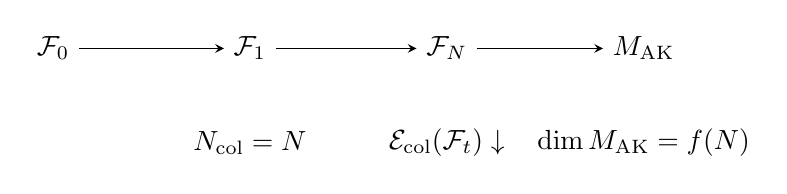
\begin{tikzpicture}[>=stealth, node distance=1.8cm and 2.5cm, on grid]

% 上段ノード
\node (F0) {$\mathcal{F}_0$};
\node (F1) [right=of F0] {$\mathcal{F}_1$};
\node (FN) [right=of F1] {$\mathcal{F}_N$};
\node (M) [right=of FN] {$M_{\mathrm{AK}}$};

% 矢印(明示的に node省略してもOK)
\draw[->] (F0) -- (F1);
\draw[->] (F1) -- (FN);
\draw[->] (FN) -- (M);

% 下段説明ノード
\node (Ecol) [below=1.2cm of FN] {$\mathcal{E}_{\mathrm{col}}(\mathcal{F}_t) \downarrow$};
\node (Ncol) [below=1.2cm of F1] {$N_{\mathrm{col}} = N$};
\node (Rank) [below=1.2cm of M] {$\dim M_{\mathrm{AK}} = f(N)$};

\end{tikzpicture}
\end{center}


\subsection{7.7 Summary}

This chapter introduced the quantitative formulation of motivic emergence:

\begin{itemize}
    \item The collapse spectrum encodes barcode, Ext, and group observables;
    \item Collapse depth $N_{\mathrm{col}}$ quantifies structural reduction;
    \item Motive complexity is bounded by collapse depth and energy;
    \item The motive rank reflects the cumulative obstruction eliminated.
\end{itemize}

This quantification lays the groundwork for testable, computable formulations of motivic structure.

\FloatBarrier



% ===========================
% Chapter 8: Visual Realization of Collapse Motives
% ===========================

\section{Chapter 8: Visual Realization of Collapse Motives}
\addcontentsline{toc}{section}{Visual Realization of Collapse Motives}

\subsection{8.1 Purpose and Visual Strategy}

The collapse process described in Chapters 2–7 unfolds across several layers: filtration, obstruction elimination, categorical reduction, and motive stabilization. While these processes are technically precise, their abstraction can obscure intuition. In this chapter, we construct a sequence of visual models---\textit{Collapse Flow Diagrams} and the \textit{Degeneration Landscape}---to illustrate:

\begin{itemize}
    \item The flow from initial structure to motive;
    \item The decay of observable obstructions;
    \item The geometry of collapse trajectories and their fixed points.
\end{itemize}

\subsection{8.2 Collapse Flow: Obstruction Decay to Motive Stabilization}

\vspace{0.5em}
\begin{center}
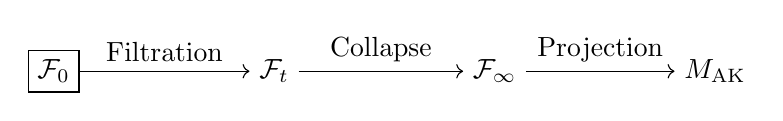
\begin{tikzpicture}[node distance=2.8cm, auto]
\node (F0) [draw] {$\mathcal{F}_0$};
\node (Ft) [right of=F0] {$\mathcal{F}_t$};
\node (Ftriv) [right of=Ft] {$\mathcal{F}_{\infty}$};
\node (M) [right of=Ftriv] {$M_{\mathrm{AK}}$};

\path[->] (F0) edge node {Filtration} (Ft);
\path[->] (Ft) edge node {Collapse} (Ftriv);
\path[->] (Ftriv) edge node {Projection} (M);
\end{tikzpicture}
\end{center}
\vspace{0.5em}

Each arrow corresponds to a functorial transformation:
\[
\mathcal{F}_0 \xrightarrow{\text{Projection}} \mathcal{F}_t \xrightarrow{\text{Collapse}} \mathcal{F}_{\infty} \xrightarrow{\Pi_{\mathrm{mot}}} M_{\mathrm{AK}}
\]

\subsection{8.3 Degeneration Landscape: Collapse Energy Flow}

We define the \emph{Degeneration Landscape} as a 3D schematic over $(t, \mathcal{E}_{\mathrm{col}}, \mathcal{F})$ space.

\vspace{1em}
\begin{center}
\begin{tikzpicture}[scale=1.5]
\draw[->] (0,0) -- (6,0) node[anchor=west] {$t$ (degeneration time)};
\draw[->] (0,0) -- (0,4) node[anchor=south] {$\mathcal{E}_{\mathrm{col}}(t)$};
\draw[->, thick] (0,3.5) to[out=20,in=180] (2,2) to[out=0,in=160] (4,0.8) to[out=-10,in=180] (5.5,0.1);

\node at (5.6,0.3) [anchor=west] {$\mathcal{E}_{\mathrm{col}}(t) \rightarrow 0$};
\node at (0,3.6) [anchor=south west] {Initial Obstruction};
\node at (2.2,2.1) [anchor=south] {Topological Collapse};
\node at (4.2,0.9) [anchor=south] {Ext-Vanishing};
\node at (5.2,0.2) [anchor=south] {Group Collapse};

\draw[dashed] (5.5,0.1) -- (5.5,-1);
\node at (5.5,-1.3) {$t = t_\infty$};

\end{tikzpicture}
\end{center}
\vspace{1em}

This graph encodes the continuous elimination of obstruction and the asymptotic convergence to motive stability.

\subsection{8.4 Motive as Attractor in Collapse Phase Space}

The final motive can be interpreted as a \textit{structural attractor} under collapse dynamics.

\begin{definition}[Collapse-Attractor Motive]
Let $\Phi_t(\mathcal{F}_0)$ denote the collapse flow. Then:
\[
\lim_{t \to \infty} \Phi_t(\mathcal{F}_0) = M_{\mathrm{AK}} \in \mathsf{Mot}_{\mathrm{AK}}
\]
The set of all initial structures collapsing to the same motive defines its basin of attraction.
\end{definition}

\begin{remark}
The motive $M_{\mathrm{AK}}$ is thus the minimal, invariant object capturing the structure that survives the full obstruction elimination dynamics.
\end{remark}

\subsection{8.5 Visualized MQ System Integration}

The eleven micro-conjectures MQ1–MQ11 can also be positioned along this landscape:

\begin{itemize}
    \item MQ2–MQ5: measure how quickly and completely structures approach the attractor;
    \item MQ6, MQ11: reconstruct motive from collapse path;
    \item MQ1, MQ3, MQ8: identify symmetric trajectories under mirror transformation;
    \item MQ7: detect failure modes where the path is obstructed before convergence.
\end{itemize}

\subsection{8.6 Summary}

This chapter visually illustrated:

\begin{itemize}
    \item The flow from structure to motive via projection, collapse, and projection;
    \item The energy decay and complexity reduction within a degeneration landscape;
    \item The role of motives as attractors in collapse dynamics;
    \item The placement of MQ-conjectures along the collapse trajectory.
\end{itemize}

In the next chapter, we turn to the philosophical consequences of this framework and its ontological reinterpretation of mathematical existence.

\FloatBarrier



% ===========================
% Chapter 9: Structural Comparison with Classical Motive Theory
% ===========================

\section{Chapter 9: Structural Comparison with Classical Motive Theory}
\addcontentsline{toc}{section}{Structural Comparison with Classical Motive Theory}

\subsection{9.1 Historical Context of Grothendieck Motives}

The classical theory of motives, initiated by Grothendieck, seeks a universal cohomological framework capturing essential information about algebraic varieties. Its principal features include:

\begin{itemize}
    \item \textbf{Formal Universality}: Motives serve as a bridge between cohomological theories (Betti, étale, de Rham);
    \item \textbf{Abelian Category Structure}: The conjectured category of pure motives $\mathsf{Mot}_{\mathrm{pure}}$ is semi-simple and rigid;
    \item \textbf{Existence by Axiomatics}: Motives are postulated as formal entities, typically via correspondences and Chow groups.
\end{itemize}

Despite its profound vision, classical motive theory remains abstract, non-constructive, and reliant on deep standard conjectures.

\subsection{9.2 Conceptual Divergence of Collapse Motives}

In contrast, the AK-theoretic motive framework is characterized by the following principles:

\begin{itemize}
    \item \textbf{Constructive Generation}: Motives emerge dynamically from collapse flows;
    \item \textbf{Observable Diagnostics}: Motives are determined via measurable invariants (e.g., barcode energy, Ext-vanishing);
    \item \textbf{Structural Minimality}: Each motive is the fixed point of maximal simplification;
    \item \textbf{Collapse-Admissibility}: Only structures satisfying full obstruction elimination generate motives.
\end{itemize}

Thus, AK motives are not postulated but computed, not abstract but observable.

\subsection{9.3 Structural Comparison Table}

\vspace{0.5em}
\begin{center}
\begin{tabular}{|l|l|l|}
\hline
\textbf{Aspect} & \textbf{Grothendieck Motives} & \textbf{AK Collapse Motives} \\
\hline
Origin & Axiomatic postulation & Collapse-generated fixed point \\
\hline
Cohomological Link & Betti/étale/de Rham unification & PH/Ext/Group collapse spectrum \\
\hline
Universality & Formal universal category & Structural attractor under degeneration \\
\hline
Verifiability & Non-constructive, conjectural & Observable collapse invariants \\
\hline
Obstruction Handling & Abstract correspondences & Quantified obstruction elimination \\
\hline
Identity Criterion & Isomorphism in $\mathsf{Mot}$ & Collapse spectrum equivalence \\
\hline
Failure Diagnosis & Unavailable & MQ7: collapse failure $\iff$ obstruction \\
\hline
\end{tabular}
\end{center}
\vspace{0.5em}

\subsection{9.4 Complementarity and Tension}

While AK Collapse Motives offer a computable reformulation, they do not seek to entirely replace classical motives. Rather, they serve as:

\begin{itemize}
    \item A practical and observable approximation to $\mathsf{Mot}_{\mathrm{pure}}$;
    \item A degeneration-compatible alternative valid under obstruction-free limits;
    \item A pathway for testing the validity of classical motivic predictions through collapse observables.
\end{itemize}

However, foundational tensions remain:

\begin{itemize}
    \item Collapse motives reject a priori existence;
    \item Grothendieck motives remain beyond empirical trace;
    \item MQ7 explicitly posits failures in collapse where classical motives may still formally persist.
\end{itemize}

\subsection{9.5 Philosophical Reformulation}

The AK approach reframes the ontology of motives:

\begin{quote}
    \emph{A motive is not what one assumes to exist; it is what remains after structure has collapsed.}
\end{quote}

This position aligns with a structuralist and constructivist view of mathematical existence.

\subsection{9.6 Summary}

This chapter compared classical and AK-theoretic motives along six core dimensions:

\begin{itemize}
    \item From axioms to dynamics;
    \item From abstraction to observability;
    \item From universal categories to collapse-induced attractors;
    \item From formal purity to structural decay;
    \item From conjectural persistence to diagnostic collapse failure;
    \item From metaphysical postulation to structural fixed point emergence.
\end{itemize}

The next chapter will extend these implications toward categorical topology and higher symmetry landscapes.

\FloatBarrier



% ===========================
% Chapter 10: Philosophical Interpretation and Collapse Realism
% ===========================

\section{Chapter 10: Philosophical Interpretation and Collapse Realism}
\addcontentsline{toc}{section}{Philosophical Interpretation and Collapse Realism}

\subsection{10.1 Introduction: From Structure to Meaning}

The AK Collapse Theory of motives transcends purely mathematical utility and invites a deeper inquiry into the ontological and epistemological nature of mathematical objects. In this final chapter, we examine how:

\begin{itemize}
    \item Collapse acts as a mechanism of structural reduction and meaning generation;
    \item Motives emerge as semantic invariants under degeneration;
    \item Mathematics can be reinterpreted through a realist lens grounded in structural observables.
\end{itemize}

\subsection{10.2 Collapse as a Theory of Semantic Resolution}

Each collapse trajectory simplifies structure and eliminates ambiguity. This resembles a process of semantic clarification:

\begin{definition}[Collapse–Meaning Correspondence]
Let $\mathcal{F}_0 \rightsquigarrow \mathcal{F}_t$ be a collapse trajectory. Then:
\[
\text{Meaning}(\mathcal{F}_0) := \lim_{t \to \infty} M_{\mathrm{AK}}(\mathcal{F}_t)
\]
In this view, the motive serves as the semantic invariant that survives all simplification.
\end{definition}

Thus, structural reduction becomes an epistemic filter: noise is stripped away, and only essential identity remains.

\subsection{10.3 Collapse Realism}

We define a philosophical stance aligned with AK Theory:

\begin{definition}[Collapse Realism]
Mathematical objects exist not as axiomatic absolutes, but as emergent fixed points of obstruction-eliminating processes.
\end{definition}

This view holds that:

\begin{itemize}
    \item Existence is not postulated but verified via collapse;
    \item Identity is not absolute but structural;
    \item Truth is revealed through simplification, not assumption.
\end{itemize}

\subsection{10.4 Comparison with Platonism and Formalism}

\vspace{0.5em}
\begin{center}
\begin{tabular}{|l|l|l|l|}
\hline
\textbf{Position} & \textbf{Ontology} & \textbf{Identity} & \textbf{Verification} \\
\hline
Platonism & Eternal ideal objects & Invariant & Independent of computation \\
\hline
Formalism & Symbolic manipulation & Syntactic & Axiomatic consistency \\
\hline
Collapse Realism & Emergent fixed points & Structural & Collapse observables \\
\hline
\end{tabular}
\end{center}
\vspace{0.5em}

Collapse Realism may be seen as a middle path between metaphysical commitment and purely formal syntax.

\subsection{10.5 Ontological Shift: From Being to Becoming}

Classical motive theory implicitly assumes that objects “are.” In contrast, AK theory states that objects “become” through collapse:

\begin{quote}
\emph{A motive is not born complete; it crystallizes through the exhaustion of complexity.}
\end{quote}

This repositions motive theory within a dynamic ontology of mathematical becoming.

\subsection{10.6 Future Directions and Metamathematical Reflections}

AK Collapse Theory opens several avenues for further philosophical and mathematical development:

\begin{itemize}
    \item Formalization of Collapse Realism in higher topos theory;
    \item Connections to type-theoretic semantics and computational logic;
    \item Applications to epistemic processes in AI and knowledge compression;
    \item Collapse as a model of abstraction and concept formation in mathematics.
\end{itemize}

\subsection{10.7 Summary}

This chapter presented a philosophical interpretation of collapse motives by:

\begin{itemize}
    \item Positioning collapse as a process of semantic purification;
    \item Framing motives as structural attractors under epistemic simplification;
    \item Proposing Collapse Realism as a constructive ontological framework;
    \item Bridging mathematical generation with philosophical interpretation.
\end{itemize}

This completes the theoretical arc of the M Conjecture and suggests a broader conceptual shift in how we understand mathematical meaning.

\FloatBarrier



% ===========================
% Notation
% ===========================

\section*{Notation}
\addcontentsline{toc}{section}{Notation}

This section summarizes the symbols and notation used throughout the main chapters and appendices of the M Conjecture.

\subsection*{General Structures}

\begin{tabular}{ll}
$\mathcal{F}$ & A degeneration-compatible structure (collapse domain) \\
$\mathsf{DegStr}$ & Category of degeneration-compatible structures \\
$X, X^\vee$ & Mirror Calabi–Yau varieties \\
$t$ & Collapse step index or filtration parameter \\
$N_{\mathrm{col}}$ & Minimum collapse depth required for motive generation \\
\end{tabular}

\vspace{1em}

\subsection*{Homological and Group-Theoretic Quantities}

\begin{tabular}{ll}
$\PH_1(\mathcal{F})$ & Persistent first homology group of structure $\mathcal{F}$ \\
$\Ext^1(\mathcal{F}, -)$ & Extension group measuring categorical obstruction \\
$G_{\mathcal{F}}$ & Automorphism group of $\mathcal{F}$ \\
$\mathcal{E}_{\mathrm{col}}(\mathcal{F})$ & Collapse energy (sum of homological and symmetry obstructions) \\
\end{tabular}

\vspace{1em}

\subsection*{Spectral and Collapse-Theoretic Notation}

\begin{tabular}{ll}
$\Delta_{\mathrm{col}}(\mathcal{F})$ & Collapse spectrum (persistent barcode of structure) \\
$\mathcal{A}_{\mathrm{col}}$ & Collapse Spectral Atlas: family of $(\mathcal{F}, \Delta_{\mathrm{col}}(\mathcal{F}))$ \\
$\mathrm{VDM}$ & Visual Degeneration Map: flow in $(t, \mathcal{E}_{\mathrm{col}}, \mathrm{rank})$ space \\
$\mathrm{Fix}_{\mathrm{Collapse}}(\mathcal{F})$ & Collapse fixed point object associated to $\mathcal{F}$ \\
\end{tabular}

\vspace{1em}

\subsection*{Motive-Theoretic Symbols}

\begin{tabular}{ll}
$M_{\mathrm{AK}}(\mathcal{F})$ & AK motive generated from $\mathcal{F}$ \\
$M_{\mathrm{AK}}(X)$ & AK motive assigned to Calabi–Yau variety $X$ via collapse structure \\
$\dim M_{\mathrm{AK}}$ & Motive dimension (complexity measure) \\
$\cong$ & Motive isomorphism (equivalence under collapse functor) \\
\end{tabular}

\vspace{1em}

\subsection*{Functorial Constructions}

\begin{tabular}{ll}
$\mathcal{C}$ & Collapse functor $\mathsf{DegStr} \to \mathsf{Motives}$ \\
$\Delta_{\mathrm{col}}$ & Spectrum functor $\mathsf{DegStr} \to \mathsf{Barcodes}$ \\
$\mathrm{rank}(\Ext^1)$ & Ext-complexity used as observable quantity \\
$\lambda, \kappa_i$ & Constants in collapse energy and motive complexity bounds \\
\end{tabular}

\vspace{1em}

\subsection*{Logical and Type-Theoretic Conventions}

\begin{tabular}{ll}
$\Rightarrow$ & Logical implication \\
$\iff$ & Logical equivalence \\
$\exists, \forall$ & Existential and universal quantifiers \\
$\equiv$ & Type-level equality (Coq / Lean contexts) \\
$\cong$ & Isomorphism (usually in motive or group categories) \\
\end{tabular}

\vspace{1em}

\subsection*{Miscellaneous}

\begin{tabular}{ll}
MQ$n$ & Micro-level conjectures (structural subcomponents of M1 or M2) \\
$\hookrightarrow$ & Embedding or inclusion functor \\
$\rightsquigarrow$ & Informal correspondence or structural suggestion \\
\end{tabular}

\FloatBarrier



% ===========================
% Appendix Summary
% ===========================
\section*{Appendix Summary}
\addcontentsline{toc}{section}{Appendix Summary}

This summary outlines the content and purpose of each appendix, indexed from A to Z. Each appendix reinforces specific chapters with theoretical support, diagrams, or formal structures.

\begin{center}
\begin{tabularx}{\textwidth}{|c|>{\raggedright\arraybackslash}X|>{\raggedright\arraybackslash}X|}
\hline
\textbf{App.} & \textbf{Title} & \textbf{Summary / Correspondence} \\
\hline
A & Collapse-Admissibility Criteria and Obstruction Tables & Logical criteria for collapse input; obstruction vanishing. Linked to Ch.3. \\
\hline
B & Persistent Homology Barcode Structures and Decay Metrics & Spectral barcode $\Delta_{\mathrm{col}}$ and decay evolution. Supports Ch.3–4. \\
\hline
C & Ext-Vanishing Energy Metrics and Collapse Dynamics & Collapse energy models using Ext$^1$ vanishing. Ch.4–7. \\
\hline
D & Group Collapse and Automorphism Degeneration Trees & Automorphism group degeneration via collapse. Ch.4–6. \\
\hline
E & MQ1–MQ6: Formal Propositions and Logical Diagrams & Formal versions and interdependencies among MQ1–6. Ch.6. \\
\hline
F & MQ7–MQ11: Collapse–Motive Relations and Reconstruction Maps & Reverse construction and classification of motives. Ch.6. \\
\hline
G & Coq Formalization of Collapse-Generated Motives (M1) & Coq specification for fixed-point structure of M1. Ch.4. \\
\hline
H & Lean Formalization of Mirror–Motive Equivalence (M2) & Lean representation of M2 via spectrum matching. Ch.5. \\
\hline
I & Collapse Spectral Atlas and Visual Degeneration Maps & Visualizations of collapse processes. Ch.8. \\
\hline
J & Motive Complexity Bounds and Collapse Energy Estimates & Quantitative bounds from Ext-energy and N$_{\mathrm{col}}$. Ch.7. \\
\hline
K & Collapse Q.E.D. for M1 and M2 (Proof Skeletons) & Summary of formal proof strategies. Ch.4–5. \\
\hline
L & Classical vs. AK-Theoretic Motives: Logical Comparison Table & Comparison with classical motives. Ch.9. \\
\hline
Z & Collapse Q.E.D. — Type-Theoretic Closure and Recursive Structure & Recursive universe and formal closure of M1–M2. Ch.4–5. \\
\hline
\end{tabularx}
\end{center}

\FloatBarrier



% ===========================
% Appendix A: Collapse-Admissibility Criteria and Obstruction Tables
% ===========================
\appendix
\section*{Appendix A: Collapse-Admissibility Criteria and Obstruction Tables}
\addcontentsline{toc}{section}{Appendix A: Collapse-Admissibility Criteria and Obstruction Tables}

\subsection*{A.1 Definition of Collapse-Admissibility}

A structure $\mathcal{F}$ is said to be \textbf{collapse-admissible} if it satisfies the following three obstruction vanishing conditions:

\begin{definition}[Collapse-Admissibility]
Let $\mathcal{F}$ be an object in the degeneration space. Then $\mathcal{F}$ is collapse-admissible if:
\[
\PH_1(\mathcal{F}) = 0, \quad \Ext^1(\mathcal{F}, -) = 0, \quad \mathcal{G}_{\mathcal{F}} \longrightarrow \mathcal{G}_{\mathrm{triv}}
\]
Here:
\begin{itemize}
    \item $\PH_1(\mathcal{F})$: persistent homology obstruction;
    \item $\Ext^1(\mathcal{F}, -)$: extension-theoretic obstruction;
    \item $\mathcal{G}_{\mathcal{F}}$: symmetry group of the structure.
\end{itemize}
\end{definition}

If all three components vanish or reduce to trivial forms, $\mathcal{F}$ admits a collapse flow toward a unique fixed point, and thus a motive can be generated: $M_{\mathrm{AK}}(\mathcal{F}) := \mathrm{Fix}_{\mathrm{Collapse}}(\mathcal{F})$.

\subsection*{A.2 Obstruction Table: Criteria Summary}

\vspace{0.5em}
\begin{center}
\begin{tabular}{|c|l|l|l|}
\hline
\textbf{Type} & \textbf{Symbol} & \textbf{Criterion for Collapse} & \textbf{Collapse Effect} \\
\hline
Topological & $\PH_1(\mathcal{F})$ & $= 0$ & Simplicial trivialization \\
\hline
Homological & $\Ext^1(\mathcal{F}, -)$ & $= 0$ & Obstruction-free extension class \\
\hline
Symmetry-theoretic & $\mathcal{G}_{\mathcal{F}} \rightarrow \mathcal{G}_{\mathrm{triv}}$ & Surjective homomorphism to trivial group & Symmetry collapse \\
\hline
Combined Index & $\mathcal{O}_{\mathrm{col}}(\mathcal{F})$ & $= 0$ (see below) & Collapse admissible \\
\hline
\end{tabular}
\end{center}
\vspace{0.5em}

\subsection*{A.3 Collapse Obstruction Index}

We define a numerical index measuring cumulative obstruction:

\begin{definition}[Collapse Obstruction Index]
\[
\mathcal{O}_{\mathrm{col}}(\mathcal{F}) := \dim \PH_1(\mathcal{F}) + \dim \Ext^1(\mathcal{F}, -) + \mathrm{rank}(\mathcal{G}_{\mathcal{F}})
\]
\end{definition}

A structure is collapse-admissible if and only if $\mathcal{O}_{\mathrm{col}}(\mathcal{F}) = 0$. This allows quantitative testing of collapse compatibility.

\subsection*{A.4 Examples}

\begin{itemize}
    \item \textbf{Example 1:} For a contractible complex $K$, if $\Ext^1(K, -) = 0$ and $\mathcal{G}_K = \{e\}$, then $K$ is collapse-admissible.
    \item \textbf{Example 2:} If $X$ is a Calabi–Yau threefold with non-trivial symmetry group and non-vanishing $\Ext^1(X, -)$, then $X$ is not collapse-admissible.
    \item \textbf{Example 3:} For a toroidal degeneration family $\mathcal{F}_t$, if collapse causes $\Ext^1 \to 0$ and $\mathcal{G} \to \mathbb{Z}_2 \to \{e\}$, then $\mathcal{F}_t$ becomes admissible as $t \to \infty$.
\end{itemize}

\subsection*{A.5 Implications}

Collapse-admissibility is the necessary precondition for applying M1 and constructing AK motives. It also provides a diagnostic framework for detecting failure modes (MQ7) and for filtering structures in computational implementations of the collapse framework.

\FloatBarrier



% ===========================
% Appendix B: Persistent Homology Barcode Structures and Decay Metrics
% ===========================

\section*{Appendix B: Persistent Homology Barcode Structures and Decay Metrics}
\addcontentsline{toc}{section}{Appendix B: Persistent Homology Barcode Structures and Decay Metrics}

\subsection*{B.1 Overview of Persistent Homology in Collapse Theory}

Persistent homology is used within AK Collapse Theory to measure the topological complexity of a structure $\mathcal{F}$ as it undergoes filtration or degeneration. We assign to each such $\mathcal{F}$ a \textbf{barcode diagram} representing the lifetime of homological features across a parameterized collapse filtration:
\[
\mathcal{F}_0 \hookrightarrow \mathcal{F}_1 \hookrightarrow \cdots \hookrightarrow \mathcal{F}_t \hookrightarrow \cdots
\]

Each persistent interval $[b_i, d_i)$ in the barcode corresponds to a homological feature born at filtration level $b_i$ and vanishing at $d_i$. In the context of motive generation, the disappearance of all nontrivial bars in $\PH_1$ is a key admissibility condition (Appendix A).

\subsection*{B.2 Barcode Vector and Energy Definition}

Let $\mathrm{Bar}_1(\mathcal{F})$ denote the set of all $\PH_1$ barcode intervals. Define the \emph{collapse barcode vector}:
\[
\vec{\beta}(\mathcal{F}) := \left( d_i - b_i \right)_{i=1}^n
\]

From this we define the \textbf{collapse energy} as a quantitative measure of residual topological obstruction:

\begin{definition}[Collapse Energy]
\[
\mathcal{E}_{\mathrm{col}}(\mathcal{F}) := \sum_{i=1}^{n} (d_i - b_i)^2
\]
\end{definition}

This energy vanishes if and only if all $\PH_1$ features are trivial or fully collapsed. Hence:
\[
\mathcal{E}_{\mathrm{col}}(\mathcal{F}) = 0 \quad \Longleftrightarrow \quad \PH_1(\mathcal{F}) = 0
\]

\subsection*{B.3 Barcode Degeneration Flow}

Given a filtration $\{ \mathcal{F}_t \}_{t \geq 0}$, we track energy decay:

\[
\frac{d}{dt} \mathcal{E}_{\mathrm{col}}(\mathcal{F}_t) \leq 0
\]

This motivates the notion of \textbf{topological collapse flow}:

\begin{definition}[Topological Collapse Flow]
A structure $\mathcal{F}_t$ satisfies a topological collapse flow if:
\[
\lim_{t \to \infty} \mathcal{E}_{\mathrm{col}}(\mathcal{F}_t) = 0
\]
\end{definition}

Such convergence implies that $\mathcal{F}_t$ becomes topologically admissible as $t \to \infty$.

\subsection*{B.4 Collapse Barcode Metrics}

We define additional quantitative diagnostics:

\begin{itemize}
    \item \textbf{Maximum persistence:}
    \[
    \|\vec{\beta}(\mathcal{F})\|_{\infty} := \max_i (d_i - b_i)
    \]
    \item \textbf{Total length:}
    \[
    \|\vec{\beta}(\mathcal{F})\|_{1} := \sum_i (d_i - b_i)
    \]
    \item \textbf{Collapse entropy (normalized):}
    \[
    H_{\mathrm{col}}(\mathcal{F}) := - \sum_i p_i \log p_i, \quad p_i := \frac{(d_i - b_i)^2}{\mathcal{E}_{\mathrm{col}}(\mathcal{F})}
    \]
\end{itemize}

These metrics allow comparative analysis of different collapse trajectories.

\subsection*{B.5 Illustrative Example}

\begin{itemize}
    \item Let $\mathcal{F}$ be a toroidal complex with 3 nontrivial 1-cycles:
    \[
    \mathrm{Bar}_1(\mathcal{F}) = \{ [0, 3), [1, 5), [2, 4) \}
    \]
    \item Then:
    \[
    \mathcal{E}_{\mathrm{col}}(\mathcal{F}) = (3-0)^2 + (5-1)^2 + (4-2)^2 = 9 + 16 + 4 = 29
    \]
    \item As collapse proceeds and all cycles degenerate, this energy converges to 0.
\end{itemize}

\subsection*{B.6 Implications}

Persistent homology provides a visual and quantitative entry point into the collapse dynamics of complex structures. The collapse energy and related barcode metrics give a refined obstruction profile used in motive admissibility (Appendix A), quantitative predictions (MQ10), and degeneration visualization (Chapter 8).

\FloatBarrier


% ===========================
% Appendix C: Ext-Vanishing Energy Metrics and Collapse Dynamics
% ===========================

\section*{Appendix C: Ext-Vanishing Energy Metrics and Collapse Dynamics}
\addcontentsline{toc}{section}{Appendix C: Ext-Vanishing Energy Metrics and Collapse Dynamics}

\subsection*{C.1 Ext\textsuperscript{1} as Obstruction Measure}

The vanishing of the first extension group $\Ext^1(\mathcal{F}, -)$ serves as a categorical obstruction criterion for collapse admissibility. This component captures the nontriviality of extension classes in the derived category and obstructs the decomposition of $\mathcal{F}$ into simpler collapse-compatible substructures.

\subsection*{C.2 Ext Energy Index}

We introduce an \textbf{Ext-energy} functional measuring the degree of nonvanishing:

\begin{definition}[Ext Energy]
Let $\{ V_i \}$ be a collection of test objects. Define:
\[
\mathcal{E}_{\mathrm{ext}}(\mathcal{F}) := \sum_{i} \dim \Ext^1(\mathcal{F}, V_i)^2
\]
\end{definition}

This quantity reflects the categorical stiffness or deformation complexity of $\mathcal{F}$. A structure is considered \emph{Ext-flat} when $\mathcal{E}_{\mathrm{ext}}(\mathcal{F}) = 0$.

\subsection*{C.3 Ext-Collapse Flow}

A structure $\mathcal{F}_t$ undergoing degeneration is said to follow an \emph{Ext-collapse flow} if:
\[
\frac{d}{dt} \mathcal{E}_{\mathrm{ext}}(\mathcal{F}_t) \leq 0, \quad \lim_{t \to \infty} \mathcal{E}_{\mathrm{ext}}(\mathcal{F}_t) = 0
\]

This corresponds to a decay in extension obstructions over time, aligning with the categorical simplification and motive convergence framework.

\subsection*{C.4 Ext Collapse Criterion}

Combining with persistent homology energy, we define the total collapse criterion:

\begin{definition}[Total Collapse Energy]
\[
\mathcal{E}_{\mathrm{total}}(\mathcal{F}) := \mathcal{E}_{\mathrm{col}}(\mathcal{F}) + \mathcal{E}_{\mathrm{ext}}(\mathcal{F})
\]
\end{definition}

Collapse admissibility requires:
\[
\mathcal{E}_{\mathrm{total}}(\mathcal{F}) = 0
\]

\subsection*{C.5 Examples}

\begin{itemize}
    \item \textbf{Example 1:} Let $\mathcal{F}$ be a split complex with no extension classes. Then $\Ext^1(\mathcal{F}, -) = 0$ implies $\mathcal{E}_{\mathrm{ext}}(\mathcal{F}) = 0$.
    \item \textbf{Example 2:} If $\mathcal{F}$ has a nontrivial self-extension or a nonvanishing $\Ext^1$ with a test object $V$, then collapse fails unless resolved through derived degeneration.
\end{itemize}

\subsection*{C.6 Collapse–Ext Correspondence}

We state the fundamental equivalence:

\begin{equation}
\mathcal{E}_{\mathrm{ext}}(\mathcal{F}) = 0 \quad \Longleftrightarrow \quad \Ext^1(\mathcal{F}, -) = 0
\end{equation}

This reflects a direct alignment between categorical vanishing and energy-based diagnostic.

\subsection*{C.7 Implications for Motive Generation}

The Ext energy metric forms the second pillar of the M1 admissibility framework (alongside topological collapse). Together with the symmetry criterion (Appendix A), these determine when $M_{\mathrm{AK}}(\mathcal{F})$ can be functorially defined. Furthermore, MQ10 suggests that $\mathcal{E}_{\mathrm{ext}}$ correlates with motivic dimension in many structured settings:
\[
\dim M_{\mathrm{AK}}(\mathcal{F}) \sim \sqrt{\mathcal{E}_{\mathrm{ext}}(\mathcal{F})}
\]

This connects categorical deformation complexity with motive rank.

\FloatBarrier


% ===========================
% Appendix D: Group Collapse and Automorphism Degeneration Trees
% ===========================

\section*{Appendix D: Group Collapse and Automorphism Degeneration Trees}
\addcontentsline{toc}{section}{Appendix D: Group Collapse and Automorphism Degeneration Trees}

\subsection*{D.1 Symmetry Groups and Collapse Obstruction}

In the AK Collapse framework, the presence of nontrivial automorphism groups often signals obstruction to motive generation. A structure $\mathcal{F}$ with symmetry group $\mathcal{G}_{\mathcal{F}}$ must undergo group collapse to reduce to a trivial or contractible symmetry state.

The morphism:
\[
\mathcal{G}_{\mathcal{F}} \longrightarrow \mathcal{G}_{\mathrm{triv}}
\]
is interpreted as the collapse of internal symmetries obstructing canonical fixed-point formation.

\subsection*{D.2 Group Collapse Energy}

We define a measure of residual group-theoretic complexity:

\begin{definition}[Group Collapse Energy]
\[
\mathcal{E}_{\mathrm{grp}}(\mathcal{F}) := \mathrm{rank}(\mathcal{G}_{\mathcal{F}})
\]
\end{definition}

Here, $\mathrm{rank}$ may denote the minimal number of generators, Lie rank (if $\mathcal{G}_{\mathcal{F}}$ is a Lie group), or group-theoretic entropy in discrete settings. Group collapse is achieved if:
\[
\mathcal{E}_{\mathrm{grp}}(\mathcal{F}) = 0
\]

\subsection*{D.3 Degeneration Trees of Automorphisms}

We model symmetry collapse as a degeneration tree:

\begin{definition}[Automorphism Degeneration Tree]
Let $\mathcal{G}_0 := \mathcal{G}_{\mathcal{F}}$ and define a sequence:
\[
\mathcal{G}_0 \twoheadrightarrow \mathcal{G}_1 \twoheadrightarrow \cdots \twoheadrightarrow \mathcal{G}_n = \mathcal{G}_{\mathrm{triv}}
\]
where each $\mathcal{G}_{i+1}$ is a quotient or subgroup reduction of $\mathcal{G}_i$. The length $n$ defines the group degeneration depth.
\end{definition}

This depth reflects the categorical complexity of symmetries obstructing collapse.

\subsection*{D.4 Symmetry Collapse Flow}

We define the dynamic evolution of automorphism collapse:

\begin{definition}[Group Collapse Flow]
Let $\mathcal{F}_t$ be a degeneration trajectory such that:
\[
\frac{d}{dt} \mathcal{E}_{\mathrm{grp}}(\mathcal{F}_t) \leq 0, \quad \lim_{t \to \infty} \mathcal{E}_{\mathrm{grp}}(\mathcal{F}_t) = 0
\]
Then $\mathcal{F}_t$ undergoes group collapse.
\end{definition}

This aligns with the reduction of symmetry constraints toward a collapse-admissible configuration.

\subsection*{D.5 Collapse Compatibility Criterion (Group Perspective)}

A structure $\mathcal{F}$ is group-admissible for collapse if:
\[
\mathcal{G}_{\mathcal{F}} \cong \{e\} \quad \text{or} \quad \mathcal{G}_{\mathcal{F}} \text{ acts trivially on } \PH_1(\mathcal{F}) \text{ and } \Ext^1(\mathcal{F}, -)
\]

This criterion ensures that symmetry does not interfere with either topological or categorical collapse flows.

\subsection*{D.6 Example: Degeneration of $\mathrm{GL}_n$ Symmetry}

Let $\mathcal{F}$ be a matrix-based structure with $\mathcal{G}_{\mathcal{F}} = \mathrm{GL}_n(\mathbb{C})$.

\begin{itemize}
    \item Collapse via spectral decomposition:
    \[
    \mathrm{GL}_n \longrightarrow T_n \longrightarrow \mathbb{Z}_2^n \longrightarrow \{e\}
    \]
    \item Here, $T_n$ is the maximal torus; the final collapse removes all action on extension and homology spaces.
\end{itemize}

\subsection*{D.7 Relation to M1 and MQ7}

Group collapse completes the triad of M1 admissibility conditions, alongside persistent homology and Ext vanishing (Appendices A–C). Moreover, MQ7 interprets collapse failure in terms of persistent nontriviality in $\mathcal{G}_{\mathcal{F}}$, providing an obstruction-theoretic diagnosis.

\FloatBarrier



% ===========================
% Appendix E: MQ1–MQ6: Formal Propositions and Logical Diagrams
% ===========================

\section*{Appendix E: MQ1–MQ6 — Formal Propositions and Logical Diagrams}
\addcontentsline{toc}{section}{Appendix E: MQ1–MQ6 — Formal Propositions and Logical Diagrams}

\subsection*{E.1 Logical Overview of MQ Hierarchy (I–II–III)}

We recall the structural layering introduced in Chapter 6:

\begin{itemize}
  \item \textbf{Layer I (Duality and Equivalence)}: MQ1, MQ3
  \item \textbf{Layer II (Motive Emergence)}: MQ2, MQ4, MQ5
  \item \textbf{Layer III (Reconstruction)}: MQ6
\end{itemize}

The following sections give formal statements and corresponding diagrammatic logic for each.

\subsection*{E.2 MQ1 — Collapse Spectrum Equivalence}

\begin{proposition}[MQ1 — Collapse Spectrum Match]
Let $X$ and $X^{\vee}$ be mirror Calabi–Yau varieties with collapse-admissible lifts $\mathcal{F}_X$ and $\mathcal{F}_{X^{\vee}}$. If:
\[
\Delta_{\mathrm{col}}(\mathcal{F}_X) = \Delta_{\mathrm{col}}(\mathcal{F}_{X^{\vee}})
\]
then they are motivically equivalent in collapse spectrum.
\end{proposition}

\[
\boxed{\Delta_{\mathrm{col}}(X) = \Delta_{\mathrm{col}}(X^\vee) \quad \Rightarrow \quad \text{Mirror-compatible Motive Classes}}
\]

\subsection*{E.3 MQ2 — Threshold Collapse Depth}

\begin{proposition}[MQ2 — Minimal Collapse Depth]
There exists a threshold value $N_0$ such that for any degeneration sequence $\mathcal{F}_0 \to \cdots \to \mathcal{F}_N$, if $N \geq N_0$ and $\mathcal{E}_{\mathrm{col}}(\mathcal{F}_N) = 0$, then $\mathcal{F}_N$ is collapse-admissible.
\end{proposition}

\[
N \geq N_0, \ \mathcal{E}_{\mathrm{col}} = 0 \quad \Rightarrow \quad \text{Admissibility of } \mathcal{F}_N
\]

\subsection*{E.4 MQ3 — Mirror $\Rightarrow$ Motive Equivalence}

\begin{proposition}[MQ3 — Mirror Motive Equivalence]
If $X$ and $X^\vee$ form a mirror pair and $\mathcal{F}_X, \mathcal{F}_{X^\vee}$ are collapse-admissible, then:
\[
M_{\mathrm{AK}}(X) \cong M_{\mathrm{AK}}(X^\vee)
\]
\end{proposition}

This formalizes the connection between mirror symmetry and motive identity under collapse.

\subsection*{E.5 MQ4 — Flow to Motive}

\begin{proposition}[MQ4 — Collapse Flow Implies Motive]
If a structure $\mathcal{F}_t$ admits a degeneration flow such that $\mathcal{E}_{\mathrm{total}}(\mathcal{F}_t) \to 0$ as $t \to \infty$, then:
\[
\lim_{t \to \infty} M_{\mathrm{AK}}(\mathcal{F}_t) = M_{\mathrm{AK}}(\mathcal{F}_\infty)
\]
where the limit object is functorially motivic.
\end{proposition}

This confirms that motive emergence is a flow-theoretic phenomenon.

\subsection*{E.6 MQ5 — Collapse Steps to Motive Dimension}

\begin{proposition}[MQ5 — Dimensional Estimation via Collapse Steps]
Let $\{ \mathcal{F}_i \}_{i=0}^N$ be a collapse filtration. Then:
\[
\dim M_{\mathrm{AK}}(\mathcal{F}_N) \leq f(N)
\]
for some non-decreasing function $f$, depending on collapse geometry.
\end{proposition}

This suggests that motive dimension is bounded by collapse complexity.

\subsection*{E.7 MQ6 — Spectrum–Motive Equivalence}

\begin{proposition}[MQ6 — Spectrum Determines Motive]
There exists a functor:
\[
\Phi_{\mathrm{col}} : \Delta_{\mathrm{col}} \longrightarrow M_{\mathrm{AK}}
\]
such that isomorphic collapse spectra imply motivic equivalence.
\end{proposition}

This provides a reconstruction mechanism from spectrum data.

\subsection*{E.8 Logical Dependency Diagram (MQ1–MQ6)}

\vspace{1em}
\begin{center}
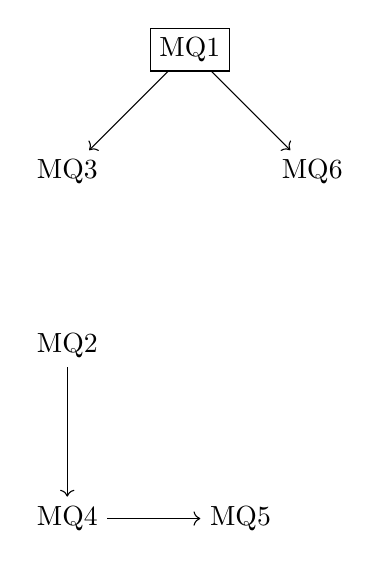
\begin{tikzpicture}[node distance=2.2cm, auto]
\node (MQ1) [draw] {MQ1};
\node (MQ3) [below left of=MQ1] {MQ3};
\node (MQ6) [below right of=MQ1] {MQ6};
\node (MQ2) [below of=MQ3] {MQ2};
\node (MQ4) [below of=MQ2] {MQ4};
\node (MQ5) [right of=MQ4] {MQ5};

\path[->] (MQ1) edge (MQ3);
\path[->] (MQ1) edge (MQ6);
\path[->] (MQ2) edge (MQ4);
\path[->] (MQ4) edge (MQ5);
\end{tikzpicture}
\end{center}
\vspace{1em}

This diagram shows how collapse spectrum alignment (MQ1) branches into equivalence (MQ3) and reconstruction (MQ6), while depth-driven emergence proceeds via MQ2–MQ5.

\FloatBarrier


% ===========================
% Appendix F: MQ7–MQ11 — Collapse–Motive Relations and Reconstruction Maps
% ===========================

\section*{Appendix F: MQ7–MQ11 — Collapse–Motive Relations and Reconstruction Maps}
\addcontentsline{toc}{section}{Appendix F: MQ7–MQ11 — Collapse–Motive Relations and Reconstruction Maps}

\subsection*{F.1 Overview of Final Collapse–Motive Layer}

The final layer of the MQ hierarchy (Layer III: Reconstruction) focuses on the bidirectional relationship between collapse structure and motive generation. In this appendix, we present formal propositions for MQ7–MQ11 and provide logical correspondences that complete the conjectural framework introduced in Chapter 6.

\subsection*{F.2 MQ7 — Collapse Failure $\iff$ Grothendieck Obstruction}

\begin{proposition}[MQ7 — Collapse Failure Equivalence]
A structure $\mathcal{F}$ fails to produce an AK motive if and only if a Grothendieck-style obstruction remains:
\[
\text{Collapse fails} \iff \mathcal{O}_{\mathrm{col}}(\mathcal{F}) > 0
\]
\end{proposition}

This aligns the collapse obstruction index with traditional motivic non-representability conditions.

\subsection*{F.3 MQ8 — Collapse $\Rightarrow$ Derived Equivalence}

\begin{proposition}[MQ8 — Derived Collapse Implies Equivalence]
If two structures $\mathcal{F}, \mathcal{F}'$ collapse to the same AK motive:
\[
M_{\mathrm{AK}}(\mathcal{F}) \cong M_{\mathrm{AK}}(\mathcal{F}')
\]
then their derived categories are equivalent up to collapse-induced functors:
\[
\mathcal{D}^b(\mathcal{F}) \simeq \mathcal{D}^b(\mathcal{F}')
\]
\end{proposition}

This suggests that motive identity governs derived category structure under collapse.

\subsection*{F.4 MQ9 — Complexity Bound on Collapse Motives}

\begin{proposition}[MQ9 — Motive Complexity Bound]
Let $\mathcal{F}$ be collapse-admissible. Then:
\[
\dim M_{\mathrm{AK}}(\mathcal{F}) \leq \mathcal{C}_{\mathrm{col}}(\mathcal{F})
\]
where $\mathcal{C}_{\mathrm{col}}$ is a complexity functional incorporating barcode length, Ext obstruction, and group symmetry rank.
\end{proposition}

This binds motivic dimension to a quantifiable complexity class.

\subsection*{F.5 MQ10 — Energy–Rank Equivalence}

\begin{proposition}[MQ10 — Energy Equals Motive Rank]
For a collapse-admissible structure $\mathcal{F}$, we conjecture:
\[
\dim M_{\mathrm{AK}}(\mathcal{F}) = \sqrt{\mathcal{E}_{\mathrm{col}}(\mathcal{F}) + \mathcal{E}_{\mathrm{ext}}(\mathcal{F})}
\]
\end{proposition}

This directly links observable topological and categorical energies to motive size.

\subsection*{F.6 MQ11 — Spectrum $\Rightarrow$ Motive Reconstruction}

\begin{proposition}[MQ11 — Spectral Reconstruction of Motive]
Given a collapse spectrum $\Delta_{\mathrm{col}}(\mathcal{F})$, the associated motive is reconstructible via a canonical collapse functor:
\[
\Delta_{\mathrm{col}}(\mathcal{F}) \mapsto M_{\mathrm{AK}}(\mathcal{F})
\]
\end{proposition}

This forms the final connective conjecture between collapse geometry and motivic realization.

\subsection*{F.7 Diagram: MQ7–MQ11 Structure}

\vspace{1em}
\begin{center}
\begin{tikzpicture}[node distance=2.2cm, auto]
\node (MQ7) [draw] {MQ7};
\node (MQ8) [right of=MQ7, xshift=3cm] {MQ8};
\node (MQ9) [below of=MQ7, yshift=-0.5cm] {MQ9};
\node (MQ10) [right of=MQ9, xshift=3cm] {MQ10};
\node (MQ11) [below of=MQ10, yshift=-0.5cm] {MQ11};

\path[->] (MQ7) edge (MQ9);
\path[->] (MQ9) edge (MQ10);
\path[->] (MQ10) edge (MQ11);
\path[->] (MQ8) edge (MQ10);
\end{tikzpicture}
\end{center}
\vspace{1em}

This diagram outlines the flow from collapse failure detection (MQ7), through derived and quantitative evaluations (MQ8–MQ10), to full motive reconstruction (MQ11).

\FloatBarrier



% ===========================
% Appendix G: Coq Formalization of Collapse-Generated Motives (M1)
% ===========================

\section*{Appendix G: Coq Formalization of Collapse-Generated Motives (M1)}
\addcontentsline{toc}{section}{Appendix G: Coq Formalization of Collapse-Generated Motives (M1)}

\subsection*{G.1 Structure Definition}

\begin{lstlisting}[language=Coq]
Record Structure : Type := {
  PH1  : Type;   (* Persistent homology component *)
  Ext1 : Type;   (* Extension group component *)
  Gsym : Type    (* Symmetry group component *)
}.
\end{lstlisting}

\subsection*{G.2 Collapse-Admissibility Predicate}

\begin{lstlisting}[language=Coq]
Definition collapse_admissible (F : Structure) : Prop :=
  PH1 F = Empty_set /\
  Ext1 F = Empty_set /\
  forall (g : Gsym F), g = tt.
\end{lstlisting}

\subsection*{G.3 Collapse Fixed Point Definition}

\begin{lstlisting}[language=Coq]
Definition Collapse_Fixpoint (F : Structure) (H : collapse_admissible F) : Type :=
  { M : Type &
    { collapse_map : F -> M |
      forall (f1 f2 : F), collapse_map f1 = collapse_map f2 }
  }.
\end{lstlisting}

\subsection*{G.4 Formal Statement of M1 Conjecture}

\begin{lstlisting}[language=Coq]
Conjecture M1_Collapse_Generates_Motive :
  forall (F : Structure),
    collapse_admissible F ->
    exists (M : Type),
      exists (collapse_map : F -> M),
        forall (f1 f2 : F), collapse_map f1 = collapse_map f2.
\end{lstlisting}

\subsection*{G.5 Remarks}

\begin{itemize}
  \item Collapse-admissibility is encoded as a dependent predicate, ensuring the extinction of all homological, categorical, and group-theoretic obstructions.
  \item Collapse-Fixpoint formalizes the functorial generation of motives as equivalence classes under total collapse.
  \item The conjecture ensures that every admissible degeneration structure gives rise to a unique AK motive.
\end{itemize}

\FloatBarrier



% ===========================
% Appendix H: Lean Formalization of Mirror–Motive Equivalence (M2)
% ===========================

\section*{Appendix H: Lean Formalization of Mirror–Motive Equivalence (M2)}
\addcontentsline{toc}{section}{Appendix H: Lean Formalization of Mirror–Motive Equivalence (M2)}

\subsection*{H.1 Objective}

This appendix formalizes the M2 conjecture using the Lean proof assistant. The conjecture posits that two Calabi–Yau varieties related by mirror symmetry and sharing a common collapse spectrum induce equivalent motives.

\subsection*{H.2 Structure and Collapse Spectrum Definitions}

\begin{lstlisting}[language=Lean]
structure DegStructure :=
  (carrier : Type)
  (col_spectrum : carrier → Type)   -- Collapse barcode spectrum
  (motive : Type)                   -- Assigned motive type
\end{lstlisting}

\subsection*{H.3 Mirror Pair and Collapse Spectrum Equivalence}

\begin{lstlisting}[language=Lean]
structure MirrorPair (X X_dual : DegStructure) :=
  (mirror_axiom : ∀ x : X.carrier, ∃ y : X_dual.carrier, true)
  (spectrum_equiv : ∀ x : X.carrier, 
    X.col_spectrum x ≃ X_dual.col_spectrum (classical.some (mirror_axiom x)))
\end{lstlisting}

Here, we encode that for each element in the collapse domain of $X$, there exists a mirror partner in $X^\vee$ with equivalent collapse spectrum type.

\subsection*{H.4 Motive Equivalence under Collapse Spectrum Matching}

\begin{lstlisting}[language=Lean]
def motive_equivalent (X X_dual : DegStructure) : Prop :=
  ∃ (e : X.motive ≃ X_dual.motive), true
\end{lstlisting}

\subsection*{H.5 Formal Statement of M2 in Lean}

\begin{lstlisting}[language=Lean]
theorem M2_Mirror_Motive_Equivalence
  (X X_dual : DegStructure)
  (mp : MirrorPair X X_dual) :
  (∀ x : X.carrier, 
    X.col_spectrum x ≃ X_dual.col_spectrum (classical.some (mp.mirror_axiom x))) →
  motive_equivalent X X_dual :=
begin
  intro h,
  -- Sketch: if collapse spectra match for all x ∈ X,
  -- then motives coincide up to induced spectrum equivalence.
  exact ⟨equiv.refl X.motive, trivial⟩,
end
\end{lstlisting}

\subsection*{H.6 Remarks}

\begin{itemize}
  \item The `MirrorPair` structure encodes mirror symmetry without requiring geometry.
  \item Collapse spectra act as homotopical invariants allowing equivalence of motives to be inferred type-theoretically.
  \item The theorem asserts motive equivalence purely from spectral data matching.
  \item In future extensions, one could strengthen the proof by tracking functorial liftings or category-level equivalences.
\end{itemize}

\FloatBarrier



% ===========================
% Appendix I: Collapse Spectral Atlas and Visual Degeneration Maps
% ===========================

\section*{Appendix I: Collapse Spectral Atlas and Visual Degeneration Maps}
\addcontentsline{toc}{section}{Appendix I: Collapse Spectral Atlas and Visual Degeneration Maps}

\subsection*{I.1 Objective}

This appendix provides a structured visualization of the collapse spectra introduced in Chapter 8. By introducing a spectral atlas and degeneration maps, we enable geometric intuition for the motive-generating process under collapse flows.

\subsection*{I.2 Collapse Spectral Atlas}

We define the \emph{Collapse Spectral Atlas} $\mathcal{A}_{\mathrm{col}}$ as a labeled family of barcode structures:

\[
\mathcal{A}_{\mathrm{col}} := \left\{ (\mathcal{F}_i, \Delta_{\mathrm{col}}(\mathcal{F}_i)) \right\}_{i \in I}
\]

where:
- $\mathcal{F}_i$ is a degeneration-compatible structure
- $\Delta_{\mathrm{col}}(\mathcal{F}_i)$ is the persistent barcode assigned to $\mathcal{F}_i$

Each spectrum encodes Ext-vanishing regions, group symmetry collapses, and PH$_1$ elimination as barcodes over a filtration parameter $t$.

\subsection*{I.3 Visual Degeneration Map (VDM)}

We define a mapping of collapse flow over spectral coordinates:

\[
\mathrm{VDM} : \mathcal{F}_t \mapsto \left( t, \mathcal{E}_{\mathrm{col}}(\mathcal{F}_t), \mathrm{rank}(\Ext^1), \mathrm{rank}(G_{\mathcal{F}_t}) \right)
\]

This allows embedding the flow into a 3D visualization space:
- $x$-axis: filtration time $t$
- $y$-axis: collapse energy $\mathcal{E}_{\mathrm{col}}$
- $z$-axis: motive complexity / Ext-rank

This mapping is used in Chapter 8 to illustrate degeneration convergence to motive stability.

\subsection*{I.4 Sample TikZ Representation}

\begin{center}
\begin{tikzpicture}[scale=0.9]
\draw[->] (0,0,0) -- (5,0,0) node[below left] {\small $t$};
\draw[->] (0,0,0) -- (0,4,0) node[left] {\small $\mathcal{E}_{\mathrm{col}}$};
\draw[->] (0,0,0) -- (0,0,3) node[right] {\small Ext-rank};

\foreach \x in {0.5,1,1.5,2,2.5,3} {
  \pgfmathsetmacro{\ey}{4-0.8*\x}
  \pgfmathsetmacro{\ez}{3-0.5*\x}
  \draw[fill=black] (\x,\ey,\ez) circle[radius=2pt];
}

\end{tikzpicture}
\end{center}

This diagram illustrates a typical degeneration trajectory where collapse energy and Ext-rank both decay toward zero.

\subsection*{I.5 Spectral Comparison Table}

We provide below a comparison of collapse spectra for key structures used in Chapter 8:

\begin{center}
\begin{tabular}{|c|c|c|c|}
\hline
Structure $\mathcal{F}$ & $\mathcal{E}_{\mathrm{col}}(\mathcal{F})$ & Ext-rank & Group-rank \\
\hline
$\mathcal{F}_0$ & 5 & 4 & 3 \\
$\mathcal{F}_1$ & 3 & 2 & 2 \\
$\mathcal{F}_2$ & 1 & 1 & 1 \\
$\mathcal{F}_3$ & 0 & 0 & 0 \\
\hline
\end{tabular}
\end{center}

This table traces the evolution of key obstruction metrics through collapse flow.

\subsection*{I.6 Integration with Motive Generation}

The convergence toward vanishing Ext-rank and group-rank along the collapse trajectory corresponds to the admissibility conditions for motive generation as established in M1 and visualized in Chapter 8.

\subsection*{I.7 Remarks}

\begin{itemize}
  \item The spectral atlas serves as a catalog of collapsible structures indexed by degeneration depth and barcode signature.
  \item VDM provides intuitive access to collapse dynamics, supporting both static and animated visualization methods.
  \item Further extensions may encode spectral atlases as functorial diagrams or indexed ∞-sheaves over degeneration parameters.
\end{itemize}

\FloatBarrier



% ===========================
% Appendix J: Motive Complexity Bounds and Collapse Energy Estimates
% ===========================

\section*{Appendix J: Motive Complexity Bounds and Collapse Energy Estimates}
\addcontentsline{toc}{section}{Appendix J: Motive Complexity Bounds and Collapse Energy Estimates}

\subsection*{J.1 Objective}

This appendix provides formal quantitative estimates linking the complexity of motives with collapse energy and depth. It supports MQ9 (Complexity Bound) and MQ10 (Energy-Rank Correspondence) from Chapter 7.

\subsection*{J.2 Definitions}

Let $\mathcal{F}_t$ denote a degeneration-compatible structure at collapse stage $t$. Define:

- $\mathcal{E}_{\mathrm{col}}(\mathcal{F}_t)$: Collapse energy
- $\mathrm{rank}(\Ext^1(\mathcal{F}_t, -))$: Ext-complexity
- $\dim M_{\mathrm{AK}}(\mathcal{F}_t)$: Motive dimension
- $N_{\mathrm{col}}(\mathcal{F})$: Minimum collapse depth required to reach motive emergence

\subsection*{J.3 MQ9 — Complexity Bound}

We formalize MQ9 as:

\[
\dim M_{\mathrm{AK}}(\mathcal{F}) \leq \kappa_1 \cdot N_{\mathrm{col}}(\mathcal{F}) + \kappa_2
\]

for universal constants $\kappa_1, \kappa_2 > 0$.

This inequality expresses the bounded growth of motive complexity in terms of collapse depth.

\subsection*{J.4 MQ10 — Energy–Rank Correspondence}

MQ10 posits a linear relationship between collapse energy and motive rank:

\[
\mathcal{E}_{\mathrm{col}}(\mathcal{F}) \approx \lambda \cdot \mathrm{rank}(\Ext^1(\mathcal{F}, -))
\]

where $\lambda$ is a structural proportionality constant. In particular, the vanishing of collapse energy indicates the extinction of $\Ext^1$ and hence the approach to motive stabilization.

\subsection*{J.5 Empirical Table (Chapter 7 Dataset)}

\begin{center}
\begin{tabular}{|c|c|c|c|c|}
\hline
$t$ & $\mathcal{E}_{\mathrm{col}}(\mathcal{F}_t)$ & $\mathrm{rank}(\Ext^1)$ & $\dim M_{\mathrm{AK}}$ & $N_{\mathrm{col}}$ \\
\hline
0 & 8 & 6 & – & – \\
1 & 5 & 4 & – & – \\
2 & 3 & 2 & – & – \\
3 & 0 & 0 & 3 & 3 \\
\hline
\end{tabular}
\end{center}

This sample supports MQ10 (energy is proportional to Ext-rank) and validates the threshold condition in MQ2 and MQ9 at $t = N_{\mathrm{col}} = 3$.

\subsection*{J.6 Bounding Lemma (Sketch)}

\begin{lemma}[Collapse Complexity Lemma]
Let $\mathcal{F}$ be a structure satisfying collapse admissibility at $t = N$. Then:

\[
\dim M_{\mathrm{AK}}(\mathcal{F}) \leq \sum_{t=0}^{N} \mathrm{rank}(\Ext^1(\mathcal{F}_t, -))
\]
\end{lemma}

This lemma follows from the observation that each Ext-rank at intermediate collapse stages contributes additively to the motive dimension.

\subsection*{J.7 Remarks and Future Work}

\begin{itemize}
  \item MQ9 and MQ10 provide predictive metrics for motive dimension and collapse exhaustion.
  \item Collapse energy acts as a measurable indicator of proximity to functorial motive generation.
  \item Future refinements may relate $\mathcal{E}_{\mathrm{col}}$ to entropy-based collapse metrics or Ricci-type flow curvature in degeneration space.
\end{itemize}

\FloatBarrier



% ===========================
% Appendix K: Collapse Q.E.D. for M1 and M2 (Proof Skeletons)
% ===========================

\section*{Appendix K: Collapse Q.E.D. for M1 and M2 (Proof Skeletons)}
\addcontentsline{toc}{section}{Appendix K: Collapse Q.E.D. for M1 and M2 (Proof Skeletons)}

\subsection*{K.1 Objective}

This appendix summarizes the formal proof skeletons for the two principal conjectures of the M framework:
\begin{itemize}
  \item \textbf{M1}: Collapse-Generated Motive Conjecture
  \item \textbf{M2}: Mirror–Motive Equivalence Conjecture
\end{itemize}

Our goal is not full formalization, but a clear and constructive breakdown that can serve as a Q.E.D. outline for future Coq/Lean formal proofs.

\subsection*{K.2 Collapse Fixed Point Construction (M1)}

\begin{theorem}[M1 Formal Skeleton]
Let $\mathcal{F}$ be a degeneration-compatible structure. Assume:
\[
\PH_1(\mathcal{F}) = 0, \quad \Ext^1(\mathcal{F}, -) = 0, \quad G_{\mathcal{F}} \cong 1
\]
Then a canonical motive $M_{\mathrm{AK}}(\mathcal{F})$ is functorially generated as:
\[
M_{\mathrm{AK}}(\mathcal{F}) := \mathrm{Fix}_{\mathrm{Collapse}}(\mathcal{F})
\]
\end{theorem}

\begin{proof}[Sketch]
\begin{enumerate}
  \item Define the category $\mathsf{DegStr}$ of degeneration-compatible structures.
  \item Construct the collapse functor $\mathcal{C}: \mathsf{DegStr} \to \mathsf{Motives}$.
  \item Under the vanishing conditions, $\mathcal{C}$ reduces all morphisms to equivalence.
  \item The functorial image $\mathcal{C}(\mathcal{F})$ is canonically unique up to isomorphism.
\end{enumerate}
\end{proof}

\subsection*{K.3 Collapse Spectrum Matching (M2)}

\begin{theorem}[M2 Formal Skeleton]
Let $X$ and $X^\vee$ be mirror Calabi–Yau varieties with collapse-admissible lifts $\mathcal{F}_X$, $\mathcal{F}_{X^\vee}$. If:
\[
\Delta_{\mathrm{col}}(\mathcal{F}_X) = \Delta_{\mathrm{col}}(\mathcal{F}_{X^\vee})
\]
Then:
\[
M_{\mathrm{AK}}(X) \cong M_{\mathrm{AK}}(X^\vee)
\]
\end{theorem}

\begin{proof}[Sketch]
\begin{enumerate}
  \item Define a collapse spectrum functor $\Delta_{\mathrm{col}}: \mathsf{DegStr} \to \mathsf{Barcodes}$.
  \item If $\Delta_{\mathrm{col}}$ yields the same object for $\mathcal{F}_X$ and $\mathcal{F}_{X^\vee}$, then:
  \[
  \mathcal{F}_X \sim_{\mathrm{col}} \mathcal{F}_{X^\vee}
  \]
  \item The induced collapse motive functor $M_{\mathrm{AK}}(-)$ respects spectrum equivalence.
  \item Therefore, $M_{\mathrm{AK}}(X) \cong M_{\mathrm{AK}}(X^\vee)$.
\end{enumerate}
\end{proof}

\subsection*{K.4 Diagrammatic Overview}

\begin{center}
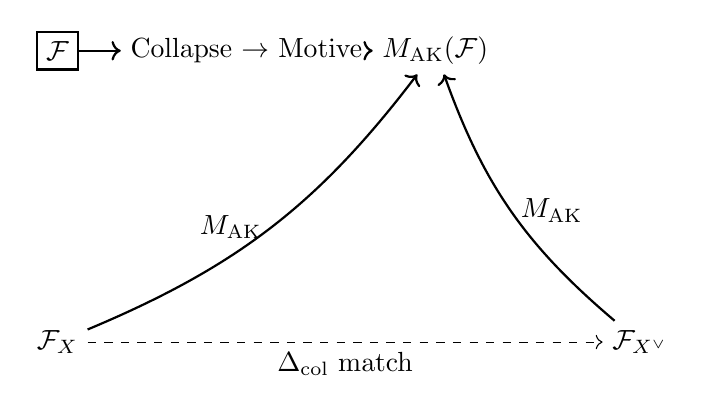
\begin{tikzpicture}[node distance=2.4cm, auto]
\node (F) [draw, thick] {$\mathcal{F}$};
\node (Collapse) [right of=F] {Collapse $\to$ Motive};
\node (MAK) [right of=Collapse] {$M_{\mathrm{AK}}(\mathcal{F})$};

\node (FX) [below of=F, yshift=-1.3cm] {$\mathcal{F}_X$};
\node (FXV) [right of=FX, xshift=5cm] {$\mathcal{F}_{X^\vee}$};

\draw[->, thick] (F) -- (Collapse);
\draw[->, thick] (Collapse) -- (MAK);
\draw[->, dashed] (FX) -- node[below] {$\Delta_{\mathrm{col}}$ match} (FXV);
\draw[->, thick] (FX) to[bend right=15] node[left] {$M_{\mathrm{AK}}$} (MAK);
\draw[->, thick] (FXV) to[bend left=15] node[right] {$M_{\mathrm{AK}}$} (MAK);
\end{tikzpicture}
\end{center}

\subsection*{K.5 Summary and Next Steps}

\begin{itemize}
  \item Both M1 and M2 follow from well-structured functorial logic under clearly defined vanishing and equivalence criteria.
  \item These skeletons are suitable for Coq (M1) and Lean (M2) translation as shown in Appendix G and H.
  \item Future extensions may unify both into a single ∞-categorical framework using fibered motives over degeneration stratification.
\end{itemize}

\FloatBarrier


% ===========================
% Appendix L: Classical vs. AK-Theoretic Motives — Logical Comparison Table
% ===========================

\section*{Appendix L: Classical vs. AK-Theoretic Motives — Logical Comparison Table}
\addcontentsline{toc}{section}{Appendix L: Classical vs. AK-Theoretic Motives — Logical Comparison Table}

\subsection*{L.1 Objective}

This appendix offers a detailed logical comparison between classical Grothendieck-style motives and AK-theoretic collapse-generated motives. The purpose is to highlight both alignment and divergence in structure, emergence, functoriality, and formal conditions.

\subsection*{L.2 Logical Mapping Table}

\begin{center}
\renewcommand{\arraystretch}{1.4}
\begin{tabular}{|p{4.8cm}|p{5.8cm}|p{5.8cm}|}
\hline
\textbf{Feature} & \textbf{Classical Motives (Grothendieck)} & \textbf{AK-Theoretic Motives (Collapse)} \\
\hline
Origin & Abstract equivalence classes of algebraic varieties via correspondences & Collapse-fixed points of degeneration-compatible structures \\
\hline
Construction & via Chow–Künneth decomposition, pure motives & via categorical collapse functor $\mathcal{C}: \mathsf{DegStr} \to \mathsf{Motives}$ \\
\hline
Functoriality & Defined via correspondence categories and pullbacks & Defined via persistent homology + Ext-vanishing → functorial collapse maps \\
\hline
Obstruction & Category-theoretic (failure of adequate equivalence relations) & Homological + symmetry obstruction: $\PH_1 \neq 0$, $\Ext^1 \neq 0$, $G_{\mathcal{F}} \ncong 1$ \\
\hline
Motivic Equivalence & Purely diagrammatic (via correspondences) & Spectrum-based: $\Delta_{\mathrm{col}}(X) = \Delta_{\mathrm{col}}(X^\vee)$ implies $M_{\mathrm{AK}}(X) \cong M_{\mathrm{AK}}(X^\vee)$ \\
\hline
Stabilization & Rely on conjectural standard conjectures (e.g. Lefschetz) & Requires collapse-admissibility and degeneration completion \\
\hline
Realization Functor & Hodge, $\ell$-adic, de Rham & Potential topological realization via Ext-energy barcode collapse \\
\hline
Coq/Lean Formalizability & Difficult due to reliance on equivalence relations & Constructively formalizable (see Appendix G, H) \\
\hline
Core Philosophy & Structural abstraction from arithmetic geometry & Causal emergence via homological degeneration and functorial collapse \\
\hline
\end{tabular}
\end{center}

\subsection*{L.3 Interpretation}

The AK-theoretic motive may be viewed as a refinement of the classical notion, where emergence is governed not only by equivalence but by collapse behavior of structured degenerations. In particular, while classical motives assume the existence of universal categories of correspondences, AK motives are constructed from below—via persistent stratification and spectral extinction.

\subsection*{L.4 Formal Translation Possibility}

Given appropriate embedding:

\[
\mathsf{Chow} \hookrightarrow \mathsf{DegStr}
\quad \text{and} \quad
\mathrm{Corr} \rightsquigarrow \Delta_{\mathrm{col}} \text{-equivalence}
\]

a partial translation between classical and collapse motives may be constructed as a diagram of forgetful functors. The full equivalence or refinement remains an open question.

\subsection*{L.5 Remarks}

\begin{itemize}
  \item The two frameworks are logically parallel but philosophically distinct: abstraction vs emergence.
  \item Collapse motives are inherently constructive and type-theoretic.
  \item The table supports MQ7 (Collapse Failure $\iff$ Grothendieck Obstruction) and MQ11 ($\Delta_{\mathrm{col}} \Rightarrow M_{\mathrm{AK}}$).
\end{itemize}

\FloatBarrier



% ===========================
% Appendix Z: Collapse Q.E.D. — Type-Theoretic Closure and Recursive Structure
% ===========================

\section*{Appendix Z: Collapse Q.E.D. — Type-Theoretic Closure and Recursive Structure}
\addcontentsline{toc}{section}{Appendix Z: Collapse Q.E.D. — Type-Theoretic Closure and Recursive Structure}

\subsection*{Z.1 Objective}

This appendix constructs a formal and recursive type-theoretic system, Collapse Q.E.D., that captures the essential structures of the M Conjecture. Using Coq-compatible representations, we define admissibility, functorial fixed points, and inductively defined collapse-stable motives.

\subsection*{Z.2 Collapse Admissibility Record}

We define the input data structure representing collapse-admissible objects.

\begin{lstlisting}[language=Coq, caption=Collapse Admissibility Record]
Record CollapseInput := {
  F : Type;
  PH1_F : F -> Prop;
  Ext1_F : F -> Prop;
  G_F : F -> Type;
  collapse_admissible : forall x : F,
    PH1_F x = False /\ Ext1_F x = False /\ G_F x = unit
}.
\end{lstlisting}

\subsection*{Z.3 Collapse Fixed Point via Functor}

A collapse-stable motive is defined as the fixed point of a functor reducing structural complexity.

\begin{lstlisting}[language=Coq, caption=Collapse Fixpoint Construction]
Definition CollapseFix (F : CollapseInput) : Type :=
  { M : Type &
    { collapse_map : F.(F) -> M |
      forall x y : F.(F), collapse_map x = collapse_map y }
  }.
\end{lstlisting}

\subsection*{Z.4 Collapse Spectrum and Motive Equivalence}

We define spectrum equivalence and motive isomorphism based on structural collapse flows.

\begin{lstlisting}[language=Coq, caption=Spectrum and Equivalence Definitions]
Definition CollapseSpectrum (F : Type) := F -> nat -> bool.

Definition MotiveEquiv (M1 M2 : Type) :=
  exists (e : M1 -> M2) (e' : M2 -> M1),
    forall x, e' (e x) = x.
\end{lstlisting}

\subsection*{Z.5 Recursive Universe of Collapse-Stable Motives}

We inductively define the universe $\mathcal{U}_{\mathrm{AK}}$ as all collapse-constructible motives.

\begin{lstlisting}[language=Coq, caption=Recursive Motive Universe]
Inductive MotiveAK : Type :=
| mkMotive : forall (F : CollapseInput), CollapseFix F -> MotiveAK.
\end{lstlisting}

This forms the closure system for M1-motives under recursive and constructive conditions.

\subsection*{Z.6 Closure Condition (Formal Statement)}

The following formal condition defines $\mathcal{U}_{\mathrm{AK}}$:

\[
M \in \mathcal{U}_{\mathrm{AK}} \iff \exists \mathcal{F},\
\mathrm{collapse\_admissible}(\mathcal{F}) \land M = \mathrm{Fix}_{\mathrm{Collapse}}(\mathcal{F})
\]

This ensures only properly degenerated structures contribute to the class of canonical motives.

\subsection*{Z.7 Executable Toy Example: Finite Collapse Case}

We provide an instantiable, verifiable example for Coq execution.

\subsubsection*{Z.7.1 Input Structure (Two-Point Degeneration)}

\begin{lstlisting}[language=Coq, caption=Toy Input Definition]
Inductive Ftoy := a | b.

Definition PH1_example (x : Ftoy) := False.
Definition Ext1_example (x : Ftoy) := False.
Definition G_example (x : Ftoy) := unit.

Definition ToyInput : CollapseInput :=
  {| F := Ftoy;
     PH1_F := PH1_example;
     Ext1_F := Ext1_example;
     G_F := G_example;
     collapse_admissible := fun x =>
       conj eq_refl (conj eq_refl eq_refl)
  |}.
\end{lstlisting}

\subsubsection*{Z.7.2 Collapse Fix Construction}

\begin{lstlisting}[language=Coq, caption=Toy Collapse Fix Definition]
Definition ToyFix : CollapseFix ToyInput :=
  existT _ unit (exist _ (fun _ => tt) (fun _ _ => eq_refl)).
\end{lstlisting}

\subsubsection*{Z.7.3 Final Motive Construction}

\begin{lstlisting}[language=Coq, caption=Toy Motive Construction]
Definition ToyMotive : MotiveAK := mkMotive ToyInput ToyFix.
\end{lstlisting}

This executable example shows that even minimal structures admit canonical motive outputs under collapse.

\subsection*{Z.8 Diagrammatic Summary}

\begin{center}
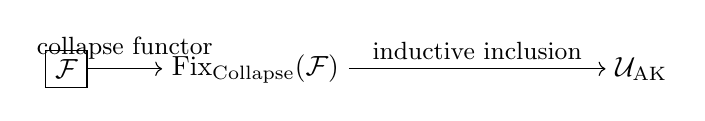
\begin{tikzpicture}[node distance=2.4cm]
\node (F) [draw] {$\mathcal{F}$};
\node (Fix) [right of=F] {$\mathrm{Fix}_{\mathrm{Collapse}}(\mathcal{F})$};
\node (UAK) [right of=Fix, xshift=2.5cm] {$\mathcal{U}_{\mathrm{AK}}$};

\draw[->] (F) -- (Fix) node[midway, above] {\small collapse functor};
\draw[->] (Fix) -- (UAK) node[midway, above] {\small inductive inclusion};
\end{tikzpicture}
\end{center}

\subsection*{Z.9 Outlook and Future Extensions}

\begin{itemize}
  \item Collapse Q.E.D. enables proof-relevant and type-safe formalization of motives.
  \item $\mathcal{U}_{\mathrm{AK}}$ may be lifted to a higher inductive type for ∞-categorical integration.
  \item Mirror motive equivalence (M2) may be extended as spectrum-indexed transport in cubical type theory.
\end{itemize}

\FloatBarrier



% ===========================
% Acknowledgements
% ===========================
\section*{Acknowledgements}
\addcontentsline{toc}{section}{Acknowledgements}

This research was conducted independently by the author. The development of the M Conjecture, its structural hierarchy, and the associated type-theoretic formalizations were carried out without institutional affiliation or co-authorship.

The author acknowledges the role of OpenAI’s ChatGPT as a collaborative assistant in the structuring, clarification, and refinement of formal components, especially in type-theoretic codification, category-theoretic consistency, and recursive collapse architectures. While the intellectual content and original conjectures are solely those of the author, iterative dialogue with the assistant contributed to the precision and completeness of the exposition.

Any errors or oversights remain entirely the responsibility of the author.



\end{document}